% ****** Start of file apssamp.tex ******
%
%   This file is part of the APS files in the REVTeX 4.1 distribution.
%   Version 4.1r of REVTeX, August 2010
%
%   Copyright (c) 2009, 2010 The American Physical Society.
%
%   See the REVTeX 4 README file for restrictions and more information.
%
% TeX'ing this file requires that you have AMS-LaTeX 2.0 installed
% as well as the rest of the prerequisites for REVTeX 4.1
%
% See the REVTeX 4 README file
% It also requires running BibTeX. The commands are as follows:
%
%  1)  latex apssamp.tex
%  2)  bibtex apssamp
%  3)  latex apssamp.tex
%  4)  latex apssamp.tex
%
\documentclass[%
reprint,
 superscriptaddress,
%groupedaddress,
%unsortedaddress,
%runinaddress,
%frontmatterverbose, 
%  preprint,
%showpacs,preprintnumbers,
%nofootinbib,
%nobibnotes,
%bibnotes,
 amsmath,amssymb,
 aps,
%pra,
%prb,
%rmp,
%prstab,
%prstper,
%floatfix,
]{revtex4-1}

\usepackage{algcompatible}
\usepackage[floatrow]{trivfloat}
\trivfloat{algorithm}
\renewcommand\algorithmname{ALGORITHM}

%\usepackage{algorithm}% http://ctan.org/pkg/algorithm
%\usepackage{algpseudocode}% http://ctan.org/pkg/algorithmicx
\usepackage{graphicx}% Include figure files
\usepackage{dcolumn}% Align table columns on decimal point
\usepackage{bm}% bold math
\usepackage{multirow}
%\usepackage{hyperref}% add hypertext capabilities
%\usepackage[mathlines]{lineno}% Enable numbering of text and display math
%\linenumbers\relax % Commence numbering lines

%\usepackage[showframe,%Uncomment any one of the following lines to test 
%%scale=0.7, marginratio={1:1, 2:3}, ignoreall,% default settings
%%text={7in,10in},centering,
%%margin=1.5in,
%%total={6.5in,8.75in}, top=1.2in, left=0.9in, includefoot,
%%height=10in,a5paper,hmargin={3cm,0.8in},
%]{geometry}
\usepackage{makecell}
\usepackage{listings}
\usepackage{longtable}
\usepackage{multirow}
\usepackage{siunitx}
\usepackage{xcolor}
%\usepackage[tableposition=top]{caption}
\usepackage{floatrow}
\floatsetup[table]{capposition=top}
\floatsetup[algorithm]{capposition=top}

\lstset{basicstyle=\ttfamily}
% \lstset{showstringspaces=false}
\lstset{columns=fullflexible}
% \lstset{keepspaces=true}
\lstset{frame=single}
\lstset{numbers=right}

\def\beq{\begin{eqnarray}}
\def\eeq{\end{eqnarray}}
\def\V{\mathcal{V}}
\def\C{\mathcal{C}}
\def\P{\mathcal{P}}

\def\NMCdiff{{N_{\mathrm{MC}}^{\mathrm{uniq}}}}
\def\Nd{{N_d}}
\def\Nddiff{{N_{d}^{\mathrm{uniq}}}}

\def\vecD{\vec{D}}
\def\veca{\vec{\alpha}}
\def\vecb{\vec{\beta}}
\def\ia{i_\alpha}
\def\ja{j_\alpha}
\def\ib{i_\beta}
\def\veciD{\vec{i}_D}
\def\vecia{\vec{i}_\alpha}
\def\vecib{\vec{i}_\beta}
\def\veciDa{\vec{i}_{D\alpha}}
\def\veciDb{\vec{i}_{D\beta}}
\def\veciaa{\vec{i}_{\alpha\alpha}}
\def\veciba{\vec{i}_{\beta\alpha}}
\def\veciab{\vec{i}_{\alpha\beta}}
\def\vecibb{\vec{i}_{\beta\beta}}

\begin{document}

%\preprint{APS/123-QED}

\title{Fast Semistochastic Heat-Bath Configuration Interaction}
% \\ or \\
% Improving the Efficiency of Semistochastic Heat-Bath Configuration Interaction \\ or \\
% Improved Semistochastic Heat-Bath Configuration Interaction Method
% Force line breaks with \\
% \thanks{J.L. and C.J.U acknowledge support from the National Science Foundation under grant ACI-1534965.}

\author{Junhao Li}
  \email{jl2922@cornell.edu}
  \affiliation{Laboratory of Atomic and Solid State Physics, Cornell University, Ithaca, New York 14853, United States}
\author{Matthew Otten}
  \email{mjo98@cornell.edu}
  \affiliation{Laboratory of Atomic and Solid State Physics, Cornell University, Ithaca, New York 14853, United States}
\author{Adam A. Holmes}
  \email{aah95@cornell.edu}
  \affiliation{Laboratory of Atomic and Solid State Physics, Cornell University, Ithaca, New York 14853, United States}
  \affiliation{Department of Chemistry and Biochemistry, University of Colorado Boulder, Boulder, Colorado 80302, United States}
 %\altaffiliation[Also at ]{Physics Department, XYZ University.}%Lines break automatically or can be forced with \\
\author{Sandeep Sharma}
  \email{sanshar@gmail.com}
  \affiliation{Department of Chemistry and Biochemistry, University of Colorado Boulder, Boulder, Colorado 80302, United States}
\author{C. J. Umrigar}%
  \email{cyrusumrigar@cornell.edu}
 %\email{Second.Author@institution.edu}
  \affiliation{Laboratory of Atomic and Solid State Physics, Cornell University, Ithaca, New York 14853, United States}


%\collaboration{MUSO Collaboration}%\noaffiliation

%\author{Charlie Author}
% \homepage{http://www.Second.institution.edu/~Charlie.Author}
%\affiliation{
% Second institution and/or address\\
% This line break forced% with \\
%}%
%\affiliation{
% Third institution, the second for Charlie Author
%}%
%\author{Delta Author}
%\affiliation{%
% Authors' institution and/or address\\
% This line break forced with \textbackslash\textbackslash
%}%

%\collaboration{CLEO Collaboration}%\noaffiliation

\date{\today}% It is always \today, today,
             %  but any date may be explicitly specified

\begin{abstract}
This paper presents in detail our fast semistochastic heat-bath configuration interaction (SHCI) method for solving the many-body Schr\"{o}dinger equation.
We identify and eliminate computational bottlenecks in both the variational and perturbative steps of the SHCI algorithm.
We also describe the parallelization and the key data structures in our implementation, such as the distributed hash table.
% To achieve high computational efficiency for large systems, we use distributed hash tables.
%The improved SHCI is blazing fast.
The improved SHCI algorithm enables us to include in our variational wavefunction two orders of magnitude more determinants
than has been reported previously with other selected configuration interaction methods.
We use our algorithm to calculate an accurate benchmark energy for the chromium dimer with the X2C relativistic Hamiltonian in the cc-pVDZ-DK basis, correlating 28 electrons in 76 spatial orbitals.
Our largest calculation uses two billion Slater determinants in the variational space, and
semistochastically includes perturbative contributions from at least trillions of additional determinants with better than $10^{-5}$~Ha statistical uncertainty.
% semistochastically includes perturbative contributions from trillions of additional determinants to obtain better than $10^{-5}$~Ha statistical uncertainty.
%Using two billion variational determinants and trillions of effective perturbative determinants, we estimate the full-CI energy of this system to be $-2099.9224(6)$~Ha.

% Our algorithm extends

% SHCI is a recently developed selected CI algorithm that can efficiently and systematically approach the full CI results and give reliable estimations of the uncertainty.
% This paper presents our latest version of SHCI comprehensively, including the key data structures, parallelization, and recent improvements that solve major bottlenecks in the original algorithm.
% We demonstrate the capability of the improved SHCI through the Cr$_2$ dimer, with active semi-core electrons and in up to a cc-pwCVQZ basis.
% The largest active space in our calculation is (28e, 288o), which gives a Hilbert space of $5.0\times10^{46}$ determinants.
% We achieve sub-millihartree accuracy for this active space in three days on eight nodes, using over a billion variational determinants and trillions of effective perturbative determinants.

%\begin{description}
%\item[Usage]
%Secondary publications and information retrieval purposes.
%\item[PACS numbers]
%May be entered using the \verb+\pacs{#1}+ command.
%\item[Structure]
%You may use the \texttt{description} environment to structure your abstract;
%use the optional argument of the \verb+\item+ command to give the category of each item. 
%\end{description}
\end{abstract}

%\pacs{Valid PACS appear here}% PACS, the Physics and Astronomy
                             % Classification Scheme.
%\keywords{Suggested keywords}%Use showkeys class option if keyword
                              %display desired
\maketitle
%\tableofcontents

\section{Introduction}
%{\color{red} I think the introduction needs a little bit more work. Right now as I see it, it is not clearly stated what the state of the art prior to the present work was and where we have taken it. To do this we should clearly distinguish what has been done before and what is new in this paper. In this regard the we have to rework paragraph 3 and 4 as I have suggested below. 
%  Paragraph 5 should, in my opinion, not be in the introduction at all. This just belongs in the result section. Below I give more thoughts on each of the paragraph in the introduction. 
%First paragraph is fine. Second paragraph compares SHCI with DMRG/FCIQMC is also fine. I think the third and fourth paragraph should be reworked. Third paragraph should further parition the two steps variational and perturbative into further sub-steps. For example variational should be partitioned into finding determinants, building Hamiltonian and diagonalizaing the Hamiltonian. PT should be split into deterministic PT and then stochastic correction to the determinisitic PT. This will allow you to then pin-point the key innovation of this paper, which is construction of the Hamiltonian and the performing a larger PT calculation deterministically. }

The choice of quantum chemistry methods requires a trade-off between accuracy and efficiency.
Density functional theory
%(DFT)~\cite{parr1979local,perdew1996generalized,kohn1999nobel}
(DFT)~\cite{ParYan-BOOK-89,DreGro-BOOK-90,kohn1999nobel}
methods with approximate density functionals
are popular and efficient, but are often not sufficiently accurate.  CCSD(T)~\cite{raghavachari1989fifth} is very accurate for single reference systems, but
not for strongly-correlated systems, such as systems with stretched bonds.
Density matrix renormalization group (DMRG)~\cite{white1993density,white1999ab,chan2002highly,chan2011density,ShaCha-JCP-12,olivares2015ab,schollwock2005density,GuoLiCha-JCTC-18}
and full configuration interaction quantum Monte Carlo (FCIQMC)~\cite{BooThoAla-JCP-09,CleBooAla-JCP-10,PetHolChaNigUmr-PRL-12,BooGruKreAla-Nat-13,HolChaUmr-JCTC-16}
are systematically improvable but rapidly get expensive with the number of electrons and the size of the basis set.

%Huron1973,BuePey-TCA-74,Evangelisti1983,cimiraglia1985second,cimiraglia1987recent,Knowles89,Har-JCP-91,povill1992treating,SteWenWilWil-CPL-94,GarCasCabMal-CPL-95,WenSteWil-IJQC-96,Neese-JCP-03,NakEha-JCP-05,AbrShe-CPL-05,BytRue-CP-09,povill1992treating,SteWenWilWil-CPL-94,GarCasCabMal-CPL-95,WenSteWil-IJQC-96,Neese-JCP-03,NakEha-JCP-05,AbrShe-CPL-05,BytRue-CP-09,Rot-PRC-09,BenAmor2011,Kno-MP-15,SchEva-JCP-16,LiuHof-JCTC-16,zhang2016deterministic,scemama2016quantum,garniron2017hybrid,giner2017jeziorski,schriber2017adaptive}

The recently developed semistochastic heat-bath configuration interaction (SHCI)~\cite{HolTubUmr-JCTC-16,ShaHolJeaAlaUmr-JCTC-17,HolUmrSha-JCP-17,SmiMusHolSha-JCTC-17,MusSha-JCTC-17,ChiHolOttUmrShaZim-JPCA-18} is another systematically improvable method capable of providing essentially exact energies for small systems.
%In common with FCIQMC, the computational cost of the method scales exponentially in the number of electrons but not in
%the number of basis functions.  However, SHCI is much faster than FCIQMC.
%The comparison with DMRG is more involved.  SHCI is often much faster than DMRG when there are many orbitals per atom.
%However, it cannot compete with DMRG for quasi 1-dimensional systems or for systems which have many natural orbitals with
%occupancies far from zero and two.
%Like FCIQMC, the computational cost of SHCI scales exponentially with the number of electrons albeit with often a
%much reduced prefactor in the exponent compared to the naive full configuration interaction (FCI), however,
%relative to FCIQMC we find that SHCI is often much cheaper in practice.
%SHCI is also often much faster than DMRG for moderately correlated systems,
%however, is much less efficient than DMRG for quasi 1-dimensional systems and even some classes of strongly correlated
%(non-quasi 1-dimensional) spin systems.
In common with FCIQMC, the computational cost of the method scales exponentially in the number of electrons but with a
much smaller exponent than in full configuration interation (FCI).  However, SHCI is much faster than FCIQMC.
The comparison with DMRG is more involved.  SHCI is often much faster than DMRG for moderately correlated systems,
however, is much less efficient than DMRG for quasi 1-dimensional systems and even some strongly correlated 
higher-dimensional spin systems. %{\color{red} which? Sandeep wanted to leave this a bit vague because it is not completely clear.}

SHCI is an example of the selected configuration interaction plus perturbation theory (SCI+PT)
%method~\cite{HurMalRan-JCP-73,BuePey-TCA-74,EvaDauMal-CP-83,Cim-JCP-85,CimPer-JCoP-87,Kno-CPL-89,Har-JCP-91,PovRubIll-TCA-92,SteWenWilWil-CPL-94,GarCasCabMal-CPL-95,WenSteWil-IJQC-96,Nee-JCP-03,NakEha-JCP-05,AbrShe-CPL-05,BytRue-CP-09,Rot-PRC-09,BenBesHoyMay-JCP-11,LiuHof-TCA-14,Eva-JCP-14,Kno-MP-15,SchEva-JCP-16,LiuHof-JCTC-16,ZhaEva-JCTC-16,SceAppGinCaf-JCoC-16,GarSceLooCaf-JCP-17,SchEva-JCTC-17,LooSceBloGarCafJac-JCP-18,TubLevHaiHeaWha-ARX-18},
methods~\cite{HurMalRan-JCP-73,BuePey-TCA-74,EvaDauMal-CP-83,CimPer-JCoP-87,Har-JCP-91,BytRue-CP-09,Eva-JCP-14,SceAppGinCaf-JCoC-16,GarSceLooCaf-JCP-17,LooSceBloGarCafJac-JCP-18,TubLevHaiHeaWha-ARX-18},
the earliest of which being
the CIPSI method~\cite{HurMalRan-JCP-73,EvaDauMal-CP-83} of Malrieu and collaborators.
SCI+PT methods have two stages.  In the first stage a variational wavefunction is constructed iteratively, starting from
%the Hartree-Fock determinant, or more generally a determinant
a determinant that is expected to have a significant amplitude in the final wavefunction, e.g., the Hartree-Fock determinant.
Each iteration of the variational stage has three steps: selection of important determinants, construction of the Hamiltonian matrix, and
iterative diagonalization of the Hamiltonian matrix.
In the second stage, 2$^{\rm nd}$-order perturbation theory is used to improve upon the variational energy.
The SHCI algorithm has greatly improved the efficiency of both stages.
First, as discussed in Section~\ref{Var}, it greatly speeds up the determinant selection, and, second, as discussed in
Section~\ref{PT}, it drastically reduces the CPU cost as well as the memory cost of performing the perturbation step by using a semistochastic algorithm.
%SHCI differs from previous SCI+PT methods in two important ways.
%First, it uses a simpler criterion for selecting determinants~\cite{HolTubUmr-JCTC-16} that avoids spending any computational time on determinants
%that do not enter in the final variational wavefunction, as well as saving time on vast numbers of determinants that make negligible perturbative contributions.
%Second, it uses a semistochastic approach~\cite{ShaHolJeaAlaUmr-JCTC-17} to perform the perturbation theory that allows one to calculate second order correction to the energy without having to simultaneously store all the determinants that contribute the the first order wavefunction, thus overcoming a severe memory bottleneck.
These two modifications have allowed SHCI to be used for systems as large as hexatriene
in an ANO-L-pVDZ basis (32 correlated electrons in 118 orbitals) which has a Hilbert space of $10^{38}$ determinants~\cite{ChiHolOttUmrShaZim-JPCA-18}.
SHCI has also recently been extended to (a) allow calculation of not just the ground state but also the low-lying excited states~\cite{HolUmrSha-JCP-17}, 
(b) allow one to perform near-exact complete active space self consistent field calculations~\cite{SmiMusHolSha-JCTC-17} by optimizing the active space orbitals and (c) include relativistic effects including the spin-orbit coupling using ``one-step" calculations with two-component Hamiltonians~\cite{MusSha-JCTC-17}.

%Since SHCI has greatly reduced the time required to select determinants, we find that for large systems the main bottlenecks
%are the time required for Hamiltonian matrix construction
%and for the stochastic part of the perturbative correction.
%For $10^8$ variational determinants, it takes two orders of magnitude more time to construct the Hamiltonian matrix than to
%find the determinants, and it may take hundreds of stochastic samples to obtain the perturbative correction with
%a statistical error of 10 $\mu$Hartree.
Since SHCI has greatly reduced the time required to select determinants, we find, for large systems, that Hamiltonian construction is the
most time-consuming step of the variational stage.
% {\color{red} semicore Cr2 in cc-pVDZ-DK? (since number of connections etc matters in timing)--Sandeep.}\\
% {\color{blue} As an order of magnitude statement, I think it is true for most molecules--Cyrus.}\\
For around $10^8$ variational determinants, it takes two orders of magnitude more time to construct the Hamiltonian matrix than to select the determinants for most molecules.
In addition, if a small stochastic error is required, the perturbative stage can be expensive,
particularly on computer systems that do not have enough memory.
Hence, in this paper, we present an improved SHCI algorithm that greatly speeds up these two steps.
For the variational stage, we introduce a fast Hamiltonian construction algorithm that allows us to use two orders of magnitude more determinants in the wavefunction.
For the perturbative stage, we introduce the 3-step batch perturbation method that further speeds up the calculation and reduces
the memory requirement.
We also describe important implementation details of the algorithm, including the key data structures and parallelization.
% We discuss the key data structures, such as the determinant and the Hamiltonian matrix representation, and the partial sums in the perturbation stage.
% We discuss the key data structures used to store the determinants, the Hamiltonian matrix and the partial sums in the perturbation stage.
% We also describe the parallelization strategy of our algorithm and illustrate the scalability of each part on modern parallel computers.

%We apply the improved SHCI to compute an accurate benchmark energy for Cr$_2$, correlating 28 electrons (valence and semicore),
%in 76 orbitals (28e, 76o), in the cc-pVDZ-DK basis.
%Cr$_2$ is a challenging system for quantum chemistry methods due to its strongly-correlated nature.
%Accurate results using smaller basis sets, or correlating only the 12 valence electrons are available, but are not
%adequate for computing a realistic potential energy curve.
%Recently DMRG and its perturbative extension (p-DMRG)~\cite{GuoLiCha-JCTC-18} have been used to calculate the ground state energy of Cr$_2$ using the same number of correlated
%electrons and the same basis as in our calculation.
%Using up to $2\times10^9$ determinants and extrapolating the total energy, we estimate the full-CI energy at equilibrium in this large active space to be $-2099.9224(6)$~Ha.
%This compares well with a p-DMRG energy of $-2099.9225$~Ha using a quadratic extrapolation.
%(The linear extrapolation used in Ref.~\onlinecite{GuoLiCha-JCTC-18} gives an energy of $-2099.9201$.)
%It should be noted that the $2\times10^9$ determinants used in our SHCI calculations are two orders of magnitude larger than the largest number of determinants
%used in any other SCI+PT method ($2\times10^7$ were used in Ref.~\cite{GarSceLooCaf-JCP-17}.)

%are the first two methods to include semi-core electrons in a cc-pVDZ basis~\cite{GuoLiCha-JCTC-18}.
%The active space of this calculation is (28e, 76o), which is exceedingly large for full-CI.
%By using SHCI with an unprecedented number of determinants and rigorous extrapolation, we achieve a significantly more accurate estimation of the full-CI energy of this large active space to be 2099.9224(6) Ha.

%The Semistochastic heat-bath configuration interaction (SHCI)~\cite{HolTubUmr-JCTC-16, ShaHolJeaAlaUmr-JCTC-17,HolUmrSha-JCP-17,SmiMusHolSha-JCTC-17,MusSha-JCTC-17}
%method is a recently developed selected configuration interaction plus perturbation theory method (SCI+PT)~\cite{HurMalRan-JCP-73,buenker1975energy,buenker1978applicability,harrison1991approximating,ben2011direct}.
%It is also essentially exact but gets expensive slower.
%SHCI differs from previous SCI+PT methods
%such as CIPSI~\cite{harrison1991approximating} in two crucial ways.
%First, whereas other methods test all determinants connected to the current wavefunction when building the variational wavefunction
%and doing the perturbation theory, SHCI looks almost only at those determinants that will be included in the variational or the perturbative spaces by using precomputed double excitation arrays~\cite{HolTubUmr-JCTC-16}.
%Second, SHCI gets around the memory bottleneck of doing large perturbative calculations by using a semistochastic approach~\cite{ShaHolJeaAlaUmr-JCTC-17}.
%SHCI has been applied to systems as large as hexatriene
%in an ANO-L-pVDZ basis, which has a Hilbert space of $10^{38}$ determinants~\cite{ChiHolOttUmrShaZim-JPCA-18}.
%It has been applied to both ground and excited states, e.g., to calculating the entire potential energy
%surfaces of the 14 lowest states of the C$_2$ molecule in up to a cc-pV5Z basis~\cite{HolTubUmr-JCTC-16}.
%
%While doing large SHCI calculations, we find the main bottlenecks of the algorithm to be the Hamiltonian matrix construction and the stochastic perturbation.
%For a hundred million variational determinants, it takes two orders of magnitude more time to construct the Hamiltonian matrix than finding these determinants. For large perturbative spaces, the stochastic part of the semistochastic perturbation can take hundreds, even thousands of iterations.
%The first contribution of this paper is to solve both of them with more efficient algorithms.
%
%We also describe important implementation details of the algorithm.
%We discuss the key data structures, such as the determinants, the Hamiltonian matrix, and the partial sums in the perturbation stage.
%We also present how we parallelize our algorithm and illustrate the scalability of each part on modern parallel computers.

%With these improvements and innovative implementation, SHCI reaches new heights in the size of the active spaces that we can calculate accurately.
%We apply the improved SHCI to Cr$_2$ in the cc-pVDZ basis to provide an accurate benchmark for this molecule in a large active space.
%Cr$_2$ is a challenging system for many quantum chemistry methods due to its strongly-correlated nature, and accurate results are only available for small active spaces, which are not sufficient for predicting some important physical quantities, such as the energy curve.
%DMRG and its perturbative extension are the first two methods to include semi-core electrons in a cc-pVDZ basis~\cite{GuoLiCha-JCTC-18}.
%The active space of this calculation is (28e, 76o), which is exceedingly large for full-CI.
%By using SHCI with an unprecedented number of determinants and rigorous extrapolation, we achieve a significantly more accurate estimation of the full-CI energy of this large active space to be 2099.9224(6) Ha.

% This paper describes in detail our latest version of SHCI.
% We discuss the key data structures, such as how we store the determinants, the Hamiltonian matrix, and the partials sums in the perturbation stage.
% We present how we parallelize SHCI, which makes it scales almost linearly to thousands of cores.
% We also make two crucial improvements to SHCI which solves it's primary bottlenecks and achieves a few orders of magnitude speedup.
% One is a more efficient algorithm for constructing the Hamiltonian matrix, and the other is the multistep batch perturbation.

We organize the paper as follows:
In section~\ref{overview}, we review the SHCI method.
In section~\ref{fast}, we introduce our faster Hamiltonian construction algorithm.
In section~\ref{multi}, we introduce our 3-step batch perturbation algorithm.
In section~\ref{key}, we describe the key data structures in our implementation.
In section~\ref{para}, we describe the parallelization strategy and demonstrate its scalability.
In section~\ref{results}, we apply our improved SHCI to Cr$_2$.
Section~\ref{conclusion} concludes the paper.

% Fast SHCI builds on SHCI and addresses two performance bottlenecks in large SHCI calculations: the construction of the sparse Hamiltonian matrix and the stochastic perturbation.

% The Hamiltonian construction becomes a bottleneck because SHCI finds important determinants much faster than previous SCI methods and can quickly go to hundreds of millions of determinants and quadrillions of Hamiltonian elements.
% Most of these elements are zero, but finding the non-zero Hamiltonian elements is a challenging task because these important determinants can have arbitrary numbers of excitations and do not exhibit any pattern in which orbitals they occupy.
% The first contribution of this work is an algorithm that can efficiently identify those non-zero Hamiltonian elements.
% This algorithm reduces the Hamiltonian construction time by order of magnitude for large calculations compared to SHCI's original algorithm.

% In addition, we develop the multistep batch perturbation which can give orders of magnitude speedup to the perturbation stage.
% In semistochastic perturbation, both the size of the deterministic perturbation and the number of samples in the stochastic perturbation have a superlinear effect on the efficiency.
% These two hyperparameters are often bounded by the system memory.
% Multistep batch perturbation allows a few orders of magnitude larger values for both of them without requiring a larger memory machine.


\section{SHCI Review}
\label{overview}
In this section, we review the semistochastic heat-bath configuration interaction method (SHCI)~\cite{HolTubUmr-JCTC-16,ShaHolJeaAlaUmr-JCTC-17,HolUmrSha-JCP-17},
emphasizing the two important ways it differs from other SCI+PT methods.
%In common with other SCI+PT methods, SHCI has two stages, the variational stage and the perturbation stage.
%{\color{red} verbatim repetition from intro:} It differs from other SCI+PT methods in three important ways.
%First, it uses a different and much faster determinant selection criterion~\cite{HolTubUmr-JCTC-16}.
%%Second, it uses ``auxiliary arrays" to speed up the calculation of the Hamiltonian matrix~\cite{ShaHolJeaAlaUmr-JCTC-17}.
%Second, it uses an efficient semistochastic algorithm to compute the perturbative correction that overcomes
%the memory bottleneck in that stage of the calculation~\cite{ShaHolJeaAlaUmr-JCTC-17}.
%(A different semistochastic algorithm has been proposed by Garniron et al.~\cite{GarSceLooCaf-JCP-17}, which is also efficient.)
In the following, we use $\V$ for the set of variational determinants, and $\P$ for the set of perturbative determinants, that is, the set of determinants that are connected to the variational determinants with a non-zero Hamiltonian matrix element but are not present in $\V$.

\subsection{Variational Stage}
\label{Var}
%{\color{red} It will be good if at some point in the description we have three bullet points for the three steps of this stage, finding determinants, constructing Hamiltonina and diagonalizing it. Then we can say that constructing hamiltonian is the step to focus on. At the end of the section one can use a simple example to say how expensive each of the steps of the variational stage are and this make the reason for working on the Hamiltonian construction easy to understand.}
%In variational stage, SHCI starts with an initial set of determinants $V_0$, usually just the Hartree-Fock determinant,
%and generates the variational wave function through an iterative process.
%
%In each iteration, we first find a set of new determinants $V'$ that connects to the current determinants set $V$.
%A new determinant $D_a$ is connected to a determinant in $V$ if and only if
%$$
%\exists D_{i} \in \V , \mathrm{s . t .} \left|H_{a i} c_{i}\right| \ge \epsilon_{1}
%$$
%where $c_i$ is the coefficient of determinant $D_i$, $H_{ai}$ is the Hamiltonian matrix element between determinant $D_a$ and $D_i$.
%$\epsilon_1$ is a small value that controls the accuracy of the variational stage.
%When $\epsilon_1=0$, it becomes a full-CI calculation.
%
%We add these new determinants into $V$, diagonalize and obtain a new set of lowest eigenvalue $E_{V}$ and eigenvector
%$\Psi_{V} = \sum_{D_{i} \in \V} c_{i} \left|D_{i}\right\rangle$.
%
%We repeat this process until the change in $E_V$ falls below a certain threshold, e.g., 1~$\mu$Ha.
%
%This process differs from other SCI methods in its criterion and the algorithm for finding new determinants.
%Conventional SCI methods often use the perturbation correction as the criteria which are expensive to evaluate,
%such as the $\left|\frac{\sum_{i} H_{a i} c_{i}}{E_{0} - H_{a a}}\right| > \epsilon_{1}$ in CIPSI~\cite{HurMalRan-JCP-73}.
%SHCI uses the much less expensive $\left|H_{a i} c_{i}\right| \ge \epsilon_{1}$ as the criterion and
%the new determinants can be found efficiently by looking up a few precomputed arrays~\cite{HolTubUmr-JCTC-16}.

SHCI starts from an initial determinant
and generates the variational wave function through an iterative process.
At each iteration, the variational wavefunction, $\Psi_V$, is written as a linear combination of the determinants in the space $\V$
\begin{align}
\Psi_{V} = \sum_{D_{i} \in \V} c_{i} \left|D_{i}\right\rangle
\end{align}
and new determinants, ${D_a}$, from the space $\P$ that satisfy the criterion
\beq
\exists D_{i} \in \V , \mathrm{\ such\ that\ } \left|H_{a i} c_{i}\right| \ge \epsilon_{1}
\label{HCI_criterion}
\eeq
are added to the $\V$ space, where
$H_{ai}$ is the Hamiltonian matrix element between determinants $D_a$ and $D_i$, and
$\epsilon_1$ is a user-defined parameter that controls the accuracy of the variational
stage~\footnote{Since the absolute values of $c_i$ for the most important determinants tends to go down as more determinants are
included in the wavefunction, a somewhat better selection of determinants is obtained by using a larger value of
$\epsilon_1$ in the initial iterations.}.
(When $\epsilon_1=0$, the method becomes equivalent to FCI.)
After adding the new determinants to $\V$, the Hamiltonian matrix is constructed, and diagonalized using the diagonally
preconditioned Davidson method~\cite{Dav-CPC-89}, to obtain an improved estimate of the lowest eigenvalue, $E_{V}$, and eigenvector, $\Psi_V$.
This process is repeated until the change in $E_V$ falls below a certain threshold, e.g., 1~$\mu$Ha.
%{\color{red} Needs clarification $\rightarrow$.}The selection of determinants is slightly better if a larger value of $\epsilon_1$ is used in the initial iterations.

Other SCI methods, such as CIPSI~\cite{HurMalRan-JCP-73,EvaDauMal-CP-83} use different criteria, usually based on either the first-order perturbative
coefficient of the wavefunction,

\beq
\left|c_a^{(1)}\right|=\left|\frac{\sum_i H_{ai}c_i}{E_0-E_a}\right| > \epsilon_1
\label{eq:cipsi_ground}
\eeq
or the second-order perturbative correction to the energy.
\beq
-\Delta E_2=-\frac{\left(\sum_i H_{ai}c_i\right)^2}{E_0-E_a} > \epsilon_1.
\label{eq:cipsi_energy}
\eeq
%which is based on a first-order perturbative estimate of the expansion coefficient.
The reason we choose instead the selection criterion in Eq.~\ref{HCI_criterion} is that it can be implemented
very efficiently without checking the vast majority of the determinants that do not meet the criterion, by taking advantage
of the fact that % the number of distinct values of the double-excitation matrix elements is only $N_{\rm orb}^4$.
most of the Hamiltonian matrix elements correspond to double excitations, and their values do not depend
on the determinants themselves but only on the four orbitals whose occupancies change during the double excitation.
Therefore, before performing an HCI run, for each pair of orbitals, the set of all double-excitation matrix elements
obtained by exciting from that pair of orbitals is computed and stored
in decreasing order by magnitude, along with the corresponding pairs of orbitals the electrons would excite to.
Then the double excitations that meet the criterion in Eq.~\ref{HCI_criterion} can be generated by
looping over all pairs of occupied orbitals in the reference determinant, and
traversing the array of sorted double-excitation matrix elements for each pair.
As soon as the cutoff is reached, the loop is exited.
Although the criterion in Eq.~\ref{HCI_criterion} is not optimal, the two selection criteria are not significantly different because
the terms in the numerator of Eq.~\ref{eq:cipsi_ground}
span many orders of magnitude, so the sum is highly correlated with the largest-magnitude term in the sum in Eq.~\ref{eq:cipsi_ground}.
It was demonstrated in Ref.~\cite{HolTubUmr-JCTC-16} that the selected determinants give only slightly inferior convergence
to those selected using the criterion in Eq.~\ref{eq:cipsi_ground}.  This is greatly outweighed by the improved selection speed.
Moreover, one could use the HCI criterion in Eq.~\ref{HCI_criterion} with a smaller value of $\epsilon_1$ as a preselection criterion, and then select determinants
using the criterion in Eq.~\ref{eq:cipsi_energy}, thereby having the benefit of both a fast selection method and a
close to optimal choice of determinants.
%{\color{red} The Aug. Berkeley paper seems to show (with one exception)
%that ASCI requires about 1.5 times fewer dets for the same energy.}

%{\color{red} If we decide not include auxiliary array as a distinguishing feature of SHCI then this paragraph can be removed.}
%SHCI also speeds up the construction of the Hamiltonian matrix.
%This is done by using $(\alpha-1)$ and $\beta$ ``auxiliary arrays" consisting of a array
%of all unique $\beta$ strings and associated with each $\beta$ string a array of all determinants in $\V$ that have that $\beta$ string, and
%a array of all unique $\alpha$ strings with $N_{\alpha}-1$ electrons and associated with each $\alpha$ string a array of all determinants in $\V$ that give the $\alpha$ string on removing one $\alpha$ electron.

%The key to the efficiency of the heat-bath scheme is as follows. The vast majority of the Hamiltonian matrix elements correspond to double excitations, and their values do not depend on the determinants themselves but only on the four orbitals whose occupancies change during the double excitation. Therefore, before performing an HCI
%run, for each pair of orbitals, the set of all double-excitation matrix elements obtained by exciting from that pair of orbitals is computed and stored
%in decreasing order by magnitude, along with the corresponding pairs of orbitals the electrons would excite to. Once this is done, at any point in the HCI algorithm, from a given reference determinant, all double excitations whose
%Hamiltonian matrix elements exceed a cutoff (either $\epsilon_1/\left|c_i\right|$ or $\epsilon_2/\left|c_i\right|$ for the variational and perturbative stages, respectively) can be generated efficiently, \emph{without having to loop over all double
%excitations}.
%% This feat
%This is achieved by looping over all pairs of occupied orbitals in the reference determinant, and
%traversing the array of sorted double-excitation matrix elements for each pair until the cutoff is reached.
%
%This screening algorithm is utilized in both steps 1a and 2a of the algorithm,
%%and is a significant reason for the speedup of the HCI algorithm over other selected CI algorithms, where it is not possible to either truncate the search for double excitations easily, or
%%to skip over the large number of determinants making negligible contributions to the energy.
%and is a significant reason why the HCI algorithm is faster than other selected CI algorithms which do not truncate the search for double excitations, or
%skip over the large number of determinants making negligible contributions to the energy.

\subsection{Perturbative Stage}
\label{PT}

In common with most other SCI+PT methods, the perturbative correction is
computed using Epstein-Nesbet perturbation theory~\cite{Eps-PR-26,Nes-PRS-55}.
The variational wavefunction is used to define the zeroth-order Hamiltonian, $H_0$ and the perturbation, $V$,
\begin{align}
H_0 &= \sum_{i,j \in \V} H_{ij} |D_i\rangle\langle D_j| + \sum_{a \notin \V } H_{aa} |D_a\rangle\langle D_a|. \nonumber\\
V &= H - H_0 . \label{eq:part}
\end{align}
The first-order energy correction is zero, and the second-order energy correction $\Delta E_{2}$ is
%The first-order correction to the wavefunction $|\Psi_1\rangle$ and the second-order
%energy correction $\Delta E_{2}$ are
%\beq
% |\Psi_1\rangle &=& \frac{1}{E_0- H_0}V|\Psi_0\rangle
% \;=\; \sum_{a} \frac{\sum_{i}H_{ai} c_i}{E_0 - E_a}  |D_a\rangle
%\eeq
%and
\beq
 \Delta E_{2} &=& \langle\Psi_0|V|\Psi_1\rangle
 \;=\; \sum_{a \in \P} \frac{\left(\sum_{i \in \V} H_{ai} c_i\right)^2}{E_0 - E_a},
\label{eq:PTa}
\eeq
where $E_a=H_{aa}$.

It is expensive to evaluate the expression in Eq.~\ref{eq:PTa} because the outer summation includes all determinants in the space $\P$ and their number is
${\cal O}(n^2v^2N_\V)$, where $N_\V$ is the number of variational determinants, $n$ is the number of electrons and $v$ is
the number of virtual orbitals. For the calculation on Cr$_2$, described in Section~\ref{results},
$n=28$, $v=62$ and $N_\V=2 \times 10^9$, so the number of determinants in $\P$ is huge.
The straightforward
and time-efficient approach to computing the perturbative correction requires storing
%and updating the partial sum for each $a$ ($\frac{\left(\sum_{i \in \V} H_{ai} c_i\right)^2}{E_0 - E_a}$) by
the partial sum $\sum_{i \in \V} H_{ai} c_i$ for each $a$, while
looping over all the determinants $i\in\V$. This creates a severe memory bottleneck.

Various schemes for improving the efficiency have been implemented, including only exciting from
a rediagonalized array of the largest-weight determinants~\cite{EvaDauMal-CP-83}, and its efficient approximation using
diagrammatic perturbation theory~\cite{CimPer-JCoP-87}.
However, this is both more complicated than necessary (requiring a double extrapolation with respect to the two
variational spaces to reach the Full CI limit) and is more computationally expensive than necessary since even
the largest weight determinants have many connections that make only small contributions to the energy.
The SHCI algorithm instead uses two other strategies to reduce both the computational time and the storage requirement.

First, SHCI screens the sum~\cite{HolTubUmr-JCTC-16} using a second threshold, $\epsilon_2$ (where $\epsilon_2<\epsilon_1$) as the criterion for selecting perturbative determinants $\P$,
\begin{equation}
%\Delta E_{2} \left(\epsilon_{2}\right) = \sum_{D_{a}} \frac{\left(\sum_{D_{i} \in \V, \left|H_{a i} c_{i}\right| \ge \epsilon_{2}} H_{a i} c_{i}\right) ^{2}}{E_{V} - H_{a a}} \\
\Delta E_{2} \left(\epsilon_{2}\right) = \sum_a \frac{\left(\sum_{D_{i} \in \V}^{(\epsilon_{2})}  H_{a i} c_{i}\right) ^{2}}{E_{V} - H_{a a}}
\label{eq:PTb}
\end{equation}
where $\sum^{(\epsilon_{2})}$ indicates that only terms in the sum for which $\left|H_{a i} c_{i}\right| \ge \epsilon_{2}$ are included.
% {\color{red} Mention that pt becomes exact when epsilon2 becomes 0. This is a good time to mention the memory bottleneck and motivate why semistochastic pt is used.}
Similar to the variational stage, we find the connected determinants efficiently with precomputed arrays of
double excitations sorted by the magnitude of their Hamiltonian matrix elements~\cite{HolTubUmr-JCTC-16}.
Note that the vast number of terms that do not meet this criterion are \emph{never evaluated}.

Even with this screening, the simultaneous storage of all terms indexed by $a$ in Eq.~\ref{eq:PTb} can exceed computer memory
when $\epsilon_2$ is chosen small enough to obtain essentially the exact perturbation energy.
The second innovation in the calculation of the SHCI perturbative correction is to overcome this memory bottleneck by
evaluating this perturbation correction semistochastically~\cite{ShaHolUmr-JCTC-17}.
The most important contributions are evaluated deterministically and the rest are sampled stochastically.
The total perturbation correction is
\beq
%\Delta E_{2} \left(\epsilon_{2}\right) = \left[\Delta E_{2} ^{\left(\mathrm{s}\right)} \left(\epsilon_{2} \right) - \Delta E_{2} ^{\left(\mathrm{s}\right)} \left(\epsilon_{2} ^{\left(\mathrm{d}\right)}\right)\right] + \Delta E_{2} ^{\left(\mathrm{d}\right)} \left(\epsilon_{2} ^{\left(\mathrm{d}\right)}\right)
\Delta E_{2} \left(\epsilon_{2}\right) = \left[\Delta E_{2} ^{\mathrm{s}} \left(\epsilon_{2} \right) - \Delta E_{2} ^{\mathrm{s}} \left(\epsilon_{2} ^{\mathrm{d}}\right)\right] + \Delta E_{2} ^{\mathrm{d}} \left(\epsilon_{2} ^{\mathrm{d}}\right)
\label{eq:semistoch_PT}
\eeq
%where $\Delta E_{2} ^{\left(\mathrm{d}\right)}$
where $\Delta E_{2} ^{\mathrm{d}}$
is the deterministic perturbation correction obtained by using a larger threshold $\epsilon_2^\mathrm{d}\ge \epsilon_2$ in Eq.~\ref{eq:PTb}.
%$\epsilon_{2} ^{\left(\mathrm{d}\right)} > \epsilon_2$.
%$\epsilon_{2} ^{\mathrm{d}} \ge \epsilon_2$.
%$\Delta E_{2} ^{\left(\mathrm{s}\right)}$
$\Delta E_{2} ^{\mathrm{s}}$
is the stochastic perturbation correction from randomly selected samples of the variational determinants, and is given by
\beq
%\Delta E_{2} ^{\left(\mathrm{s}\right)} = & \frac{1}{N_{d} \left(N_{d} - 1\right)} \left\langle \sum_{D_{a} \in \P} \left[\left(\sum_{D_i \in \V} ^{N_{d} ^{\mathrm{(unique)}}} \frac{w_{i} c_{i} H_{a i}}{p_{i}}\right) ^{2} \right. \right. \\ + 
% & \left. \left. \sum_{D_i \in \V} ^{N_{d} ^{\mathrm{(unique)}}} \left(\frac{w_{i} \left(N_{d} - 1\right)}{p_{i}} - \frac{w_{i} ^{2}}{p_{i} ^{2}}\right) c_{i} ^{2} H_{a i} ^{2}\right] \frac{1}{E_{0} - E_{a}} \right\rangle
%\Delta E_{2} ^{\mathrm{s}}(\epsilon_2)
%=& \frac{1}{N_{d} \left(N_{d} - 1\right)} \left\langle \sum_{D_{a} \in \P}^{(\epsilon_2)} \left[\left(\sum_{D_i \in \V} ^{N_{d} ^{\Nddiff}} \frac{w_{i} c_{i} H_{a i}}{p_{i}}\right) ^{2} \right. \right. \nonumber \\
%+& \left. \left. \sum_{D_i \in \V} ^{N_{d} ^{\Nddiff}} \left(\frac{w_{i} \left(N_{d} - 1\right)}{p_{i}} - \frac{w_{i} ^{2}}{p_{i} ^{2}}\right) c_{i} ^{2} H_{a i} ^{2}\right] \frac{1}{E_{0} - E_{a}} \right\rangle
\lefteqn{\!\!\!\!\!\!\!\!\Delta E_{2} ^{\mathrm{s}}(\epsilon_2) =
 \frac{1}{N_{d} \left(N_{d} - 1\right)} \left\langle \sum_{D_{a} \in \P} \left[\left(\sum_{D_i \in \V} ^{{\Nddiff}, \left(\epsilon_2\right)} \frac{w_{i} c_{i} H_{a i}}{p_{i}}\right) ^{2} \right. \right.} \nonumber \\
&&\!\!\!\!\!\!\!+ \left. \left. \sum_{D_i \in \V} ^{{\Nddiff}, \left(\epsilon_2\right)} \left(\frac{w_{i} \left(N_{d} - 1\right)}{p_{i}} - \frac{w_{i} ^{2}}{p_{i} ^{2}}\right) c_{i} ^{2} H_{a i} ^{2}\right] \frac{1}{E_{0} - E_{a}} \right\rangle
\label{eq:stoch_PT}
\eeq
where $N_d$ is the number of variational determinants per sample and
%$N_d^{\mathrm{(unique)}}$ is the number unique ones.
$\Nddiff$ is the number different determinants in a sample.
$p_i$ and $w_i$ are the probability of selecting determinant $D_i$ and the number of copies of that determinant in a
sample, respectively.
The $N_d$ determinants are sampled from the discrete probability distribution
\beq
p_{i} &=& {\left|c_{i}\right| \over \sum_j^\V \left|c_{j}\right|},
\label{sampling_prob}
\eeq
using the Alias method~\cite{walker1977efficient,kronmal1979alias}, which allows samples to be drawn
in ${\cal O}(1)$ time. (The more commonly used heatbath method requires ${\cal O}(\log(n))$ time to do a binary search of an array of cumulative probabilities.)
$\Delta E_2[\epsilon_2]$ and $\Delta E_2[\epsilon_2^{\mathrm{d}}]$ are calculated using the same set of samples,
and thus there is significant cancellation of stochastic error.
Furthermore, because these two energies are calculated simultaneously, the additional cost of performing this
calculation, compared to a purely stochastic summation, is very small.
Clearly, in the limit that $\epsilon_2^{\mathrm{d}} = \epsilon_2$, the entire perturbative calculation becomes deterministic.

The perturbative stage of the SHCI algorithm has the interesting feature that it achieves super-linear speedup with
the number of computer nodes used.  There are two reasons for this, both having to do with the increase in the total computer memory.
First, a larger fraction of the perturbative energy can be computed deterministically, using a smaller value of $\epsilon_{2} ^{\mathrm{d}}$ in Eq.~\ref{eq:semistoch_PT}.
Second, a larger value of $N_d$ in Eq.~\ref{eq:stoch_PT} can be used.
For a given total number of samples, the statistical error is smaller for a small number of large samples,
than for a large number of small samples, because the number of sampled contributions to the energy correction is a quadratic function of the number of sampled variational determinants.
Consequently, this too contributes to a super-linear speedup.

\subsection{Other features of SHCI}
\label{other_features}
We note that although SHCI has a stochastic component, it has the advantages compared to quantum Monte Carlo algorithms that there is no sign problem,
and that each sample is independent.
%Finally, a series of SHCI calculations with different values of the variational threshold $\epsilon_1$ can be performed, in order to enable
%an extrapolation to the Full CI limit ($\epsilon_1=0$).
%The extrapolation is performed by fitting a quadratic function to the total energy as a function of the perturbative correction $\Delta E$,
%  weighting each point by $\left(\Delta E\right)^{-2}$.
Another feature of the method is that if the calculation is done for various values of the variational threshold $\epsilon_1$
a plot of the total energy (variational plus perturbative correction) plotted versus the perturbative correction yields a smooth curve that can be used to assess the convergence and extrapolate to the Full CI limit,  $\Delta E=0$~\cite{HolUmrSha-JCP-17}.
%We typically do this by fitting quadratic function weighting each point by $\left(\Delta E\right)^{-2}$~\cite{ChiHolOttUmrShaZim-JPCA-18}.
We typically use a quadratic fit, with the points weighted by $\left(\Delta E\right)^{-2}$~\cite{ChiHolOttUmrShaZim-JPCA-18}.

As is typical in many quantum chemistry methods, we note that the convergence of both the variational energy and the total (variational plus perturbative) energy
depends on the choice of orbitals.  Natural orbitals, calculated within HCI, are typically a better choice than Hartree Fock orbitals,
and optimized orbitals~\cite{SmiMusHolSha-JCTC-17} are a yet better choice.  For systems with more than a few atoms,
split-localized optimized orbitals lead to yet better convergence~\cite{ChiHolOttUmrShaZim-JPCA-18}.

We describe, in the next two sections, improvements we have made to the variational and the perturbative stages of the SHCI algorithm,
which speed up the calculations by an order of magnitude or more for large systems.

\section{Fast Hamiltonian Construction}
%\subsection{Fast Hamiltonian Construction}
\label{fast}
%{\color{red} This section may need some more work. I agree. I think an algorithm in the form of a simple psuedo code or a diagram will make things much more clear.}\\

The Hamiltonian matrix is stored in upper-triangular sparse matrix form.
At each variational iteration, we have a set of old determinants, and a set of new determinants.
We have calculated the Hamiltonian matrix for the old determinants, and need to calculate the old-new and the new-new
matrix elements.

The SHCI algorithm greatly speeds up the step of finding the important determinants and one can very quickly generate
hundreds of millions or more.  With this many determinants, the construction of the Hamiltonian matrix is expensive.
Most of the matrix elements are zero, but finding the non-zero Hamiltonian elements quickly is challenging because
the determinants in the variational wavefunction do not exhibit any pattern.
(Efficient construction of the Hamiltonian matrix of the same size in FCI is much more straightforward than in SCI.)
There are two straightforward ``brute force" approaches to building the Hamiltonian matrix:
a) looping over all pairs of determinants to find those pairs that are related by single or double excitations, and, b)
generating all connections of each det and searching for them in the sorted array of variational determinants.
When the number of determinants is not very large, the former is more efficient.
Both of these are much too expensive for the very large number of variational determinants that we use.

\begin{table}[h]
\caption{The notation for the data structures in our current algorithm for efficiently constructing the Hamiltonian matrix.
Analogous data structures with the alpha and beta roles reversed are also used.
The text gives details of how they are constructed efficiently.}
\begin{tabular}{ll}
\hline
\hline
Notation& \multicolumn{1}{c}{Description}\\
\hline
%$D, D'$& Symbol for the Determinants\\
%$\alpha, \alpha'$ & Symbol for the alpha strings\\
%$\beta, \beta'$& Symbol for the beta strings\\
%$i_D$, $i_\alpha$
$\vecD$ & The array of determinants in $\V$ in the order\\
& they were generated. \\
&\\
$\veca$ & The array of all alpha strings, without repeats\\
& that are present in at least one determinant in\\
& $\V$ in the order they were generated. \\
&\\
%\{$\alpha^{(-1)}$\} & The array of all alpha strings for $n_\alpha-1$ electrons that\\
%&can be obtained by removing one electron from the \{$\alpha$\}. \\
%&\\
$\ia(\alpha)$ & Hash map that takes an alpha string, $\alpha$, \\
& and returns its index, $\ia$, in $\veca$. \\
&\\
$\veciDa(\ia)$ & The array of determinant indices in $\vecD$ such\\
& that the alpha strings of those determinants \\
& have index $\ia$ in $\veca$. \\
%$\veciDa(\ia)$ & The array of determinant indices $\veciDa$ \\
%& that have $\alpha_{\ia}$ as their alpha string. \\
%&  $i_{\alpha_i}$ is the index \\
%& of $\alpha_i$ in $\veca$.  The determinant index $i_D$ indicates \\
%& the order in which determinant $D$ was added to \\
%& the variational space $\V$. The determinant indices \\
%& in $\veciDa(i_{\alpha_i})$ are either sorted by $i_D$ or by $\ib$ \\
%& (the indices of their beta strings in $\vecb$). \\
& The elements of $\veciDa(\ia)$ are sorted either by\\
& their values, or by the indices of their beta \\
& strings in $\vecb$. (See text for details.)\\
&\\
$\veciba(\ia)$ & The array of all beta string indices in $\beta$ that\\
& appear with $\alpha_{\ia}$ in a determinant. \\
& It is sorted so that the elements of $\veciDa(\ia)$ \\
& and $\veciba(\ia)$ are always in correspondence.\\
&\\
%$\vecia(\alpha^{(-1)})$ & Hash map that gives the array of indices of \\
%& alpha strings in the array $\veca$ that can give $\alpha^{(-1)}$ \\
%& upon removing an electron.\\
%&\\
$\vecia(\alpha^{(-1)})$ & Hash map that takes an alpha string with one \\
& less electron, $\alpha^{(-1)}$, and returns an array of  \\
& indices of alpha strings in $\veca$ that can give  \\
& $\alpha^{(-1)}$ upon removing an electron.  These are \\
& generated only for the $\alpha$'s present in the new \\
& determinants.\\
% &\\
% $\vecb_{\alpha_i}$ & The array of all $\beta$ string that are coupled with\\
% & the alpha string $\alpha_i$ to give a Determinant\\
% & in the space $\V$\\
&\\
$\veciaa(j_\alpha)$ & The array of indices of alpha strings \\
& in the array $\veca$, connected by a single excitation \\
& to the $j_\alpha^{th}$ alpha string of array $\veca$, sorted \\
%& according to their indices in \{$\alpha$\}. These are \\
& in ascending order. These are \\
& generated only for the $j_\alpha$'s present in the new \\
& determinants.\\
% I sort by the indices in the unique alpha array, but I don't think we need to mention that, which will double the length of the section.
% $\veca_{\alpha_i}$ & A array of all $\alpha$ string sorted according to\\
% & their indices in \{$\alpha$\} and that are  connected to \\
% & the alpha string $\alpha_i$  by a single excitation\\
&\\
$i_D, j_D, \cdots$ & Indices of $\vecD$.\\
&\\
$\ia, j_\alpha, \cdots$ & Indices of $\veca$.\\
&\\
$\alpha(D_i)$ & Alpha string of determinant $D_i$.\\
&\\
\hline
\end{tabular}
\label{auxiliary}
\end{table}


\begin{algorithm}
\caption{Hamiltonian matrix update for determinants connected by single or double alpha excitations.
The algorithm for single or double beta excitations is very similar.
}
\begin{algorithmic}
\FOR{$D_i$ in $\vecD$}
% \State Use hash map $\ib(\beta(D_i))$ to find the index of
% \State \hskip 4mm the beta string of $D_i$ in $\vecb$
% \State $\ib$ is the index of the beta string of $D_i$ in $\vecb$
  \State Use hash map $\ib(\beta)$ to find $\ib$, the index of $\beta(D_i)$
  %\State \hskip 4mm \beta($D_i$). % in $\vecb$
  \State $s$ is the index of the first new determinant with $s \ge i$.
  \FOR{$j$ in $\veciDb(\ib)$}
  \IF{$j \geq s$ and $D_i, D_j$ are connected}
    \State Compute and add $H_{ij}$ to the Hamiltonian
  \ENDIF
  \ENDFOR
\ENDFOR
\end{algorithmic}
\label{same_spin}
\vskip 7mm
\end{algorithm}


\begin{algorithm}
%\caption{Hamiltonian matrix update for determinants connected by a single $\alpha$ and a single $\beta$ excitation.
\caption{Hamiltonian matrix update for determinants connected by an opposite-spin double excitation.
}
\begin{algorithmic}

\FOR{$D_i$ in $\vecD$}
  \State Use hash maps $\ia(\alpha)$ and $\ib(\beta)$ to find $\ia, \ib$,
  \State \hskip 4mm the indices of $\alpha(D_i)$ and $\beta(D_i)$.
% \State \hskip 4mm in $\veca$ and $\vecb$ resp.
  \State $s$ is the index of the first new determinant with $s>i$.
  \FOR{$k_\alpha$ in $\veciaa(\ia)$}
    \IF{number of new determinants is small}
%       \State $\vecD_{\alpha_k}$ is sorted by $D$
%     \FOR {$j \ge s$ in $\vecD_{\alpha_k}$ (reverse loop)}
      \FOR {$j \ge s$ in $\veciDa({k_\alpha})$ (reverse loop)}
%     \FOR {$j \ge s$ (reverse loop over $\vecD$)}
%       \State $\beta(D_j)$ is the $\beta$-string of $D_j$
%       \IF {$\beta(D_j)$ present in $\vecb_{\beta_i}$ (binary search)}
        \IF {$\ib(\beta(D_j))\in\vecibb(\ib)$ (binary search)}
          \State Compute and add $H_{ij}$ to the Hamiltonian
        \ENDIF
      \ENDFOR
    \ELSE
%       \State $\vecD_{\alpha_k}$ is sorted by $\beta$
%     \State Find the inner join $\vecD_J$ of $\vecD_{\alpha_k}$ and $\vecb_{\beta_i}$ on $\beta$ 
%     \State Find the intersection $\vec{j}_D$ of sorted arrays 
%     \State \hskip 4mm $\veciba(k_\alpha)$ and $\veciba(\ib)$ in ${\cal O}(n)$ time.
      \State Find the intersection $\vec{j}_\beta$ of sorted arrays 
      \State \hskip 4mm $\veciba(k_\alpha)$ and $\vecibb(\ib)$ in ${\cal O}(n)$ time.
      \State \hskip 4mm Since $\veciba(k_\alpha)$ and $\veciDa(k_\alpha)$ are in
      \State \hskip 4mm 1-to-1 correspondence, this provides the
      \State \hskip 4mm corresponding determinants $\vec{j}_D$
      \FOR {$j$ in $\vec{j}_D$}
        \IF {$j \ge s$}
          \State Compute and add $H_{ij}$ to the Hamiltonian
        \ENDIF
      \ENDFOR
%       \State merge two sorted array $\vecb_{\alpha_k}$ and $\{\beta\}_{\beta_i}$
    \ENDIF
  \ENDFOR
\ENDFOR

%\\
%\FOR{$D_i$ in $\V$}
%  \State $\alpha_i$ is the $\alpha$-string of $D_i$
%  \State $\beta_i$ is the $\beta$-string of $D_i$
%  \State $D_s$ is first new determinant larger than $D_i$
%  \FOR {$\alpha_k$ in $\veca_{\alpha_i}$}
%    \IF{number of new determinants is small}
%%       \State $\vecD_{\alpha_k}$ is sorted by $D$
%      \FOR {$D_j$ larger than $D_s$ in $\vecD_{\alpha_k}$ (reverse loop)}
%        \State $\beta_j$ is the $\beta$-string of $D_j$
%        \IF {$\beta_j$ present in $\vecb_{\beta_i}$ (binary search)}
%          \State Add $H_{ij}$ to the sparse matrix
%        \ENDIF
%      \ENDFOR
%    \ELSE
%%       \State $\vecD_{\alpha_k}$ is sorted by $\beta$
%      \State Find the inner join $\vecD_J$ of $\vecD_{\alpha_k}$ and $\vecb_{\beta_i}$ on $\beta$ 
%      \FOR {$D_j$ in $\vecD_J$}
%        \IF {$D_j > D_s$}
%          \State Add $H_{ij}$ to the sparse matrix
%        \ENDIF
%      \ENDFOR
%%       \State merge two sorted array $\vecb_{\alpha_k}$ and $\{\beta\}_{\beta_i}$
%    \ENDIF
%  \ENDFOR
%\ENDFOR
%\\
%
%\FOR{$D$ in $\V$}
%  \State $\alpha$ is the alpha-string of $D$
%  \State $\beta$ is the beta-string of $D$
%  \State $D''$ is first new determinant such that $i_{D''} \geq i_{D}$
%  \FOR {$\alpha'$ in $\veca_{\alpha}$}
%    \IF{number of new determinants is small}
%%       \State $\vecD_{\alpha_k}$ is sorted by $D$
%      \FOR {$D'$ larger than $D''$ in $\vecD_{\alpha'}$ (reverse loop)}
%        \State $\beta'$ is the beta-string of $D'$
%        \IF {$\beta'$ present in $\vecb_{\beta}$ (binary search)}
%          \State Add $\langle D' |H|D\rangle$ to the sparse matrix
%        \ENDIF
%      \ENDFOR
%    \ELSE
%%       \State $\vecD_{\alpha_k}$ is sorted by $\beta$
%      \State Find the inner join $\vecD_J$ of $\vecD_{\alpha'}$ and $\vecb_{\beta}$ on $\beta$ 
%      \FOR {$D'$ in $\vecD_J$}
%        \IF {$i_{D'} > i_{D''}$}
%          \State Add $\langle D' |H|D\rangle$ to the sparse matrix
%        \ENDIF
%      \ENDFOR
%%       \State merge two sorted array $\vecb_{\alpha_k}$ and $\{\beta\}_{\beta_i}$
%    \ENDIF
%  \ENDFOR
%\ENDFOR

% \FOR{$\alpha_i$ in \{$\alpha$\}}
% 	\FOR{$D_i$ in $\vecD_{\alpha_i}$ }
%     \State $\alpha_i$ is the $\alpha$-string of $D_i$
%     \State $\beta_i$ is the $\beta$-string of $D_i$
% 	\FOR {$\alpha_k$ in $\veca_{\alpha_i}$}
%     \FOR {$\beta_l$ in $\vecb_{\alpha_k}$}
%     \IF {$\beta_l$ present in $\vecb_{\beta_i}$ (binary search)}
%      \State $D_k$ is the determinant ($\alpha_k$)($\beta_l$) 
%      \State Add $H_{ik}$ to the sparse matrix if $D_i > D_k$
%      \ENDIF
%      \ENDFOR
%     \ENDFOR
% \ENDFOR
% \ENDFOR
\end{algorithmic}
\label{opposite_spin}
\end{algorithm}

The original SHCI algorithm introduced
%the $\alpha-1, \beta$ ``auxiliary arrays" method~\cite{ShaHolJeaAlaUmr-JCTC-17},
%which is much faster than brute force but still spends considerable time on elements that are zero.
%Here, we extend the $\alpha-1,\beta$ method, to further reduce the time spent on zero elements.
auxiliary arrays~\cite{ShaHolJeaAlaUmr-JCTC-17} to speed up the Hamiltonian construction,
but it still spends considerable time on elements that are zero.
In our improved SHCI algorithm, we use a larger number of auxiliary arrays to further reduce the time.
All the relevant data structures are shown in Table~\ref{auxiliary}.
%spent on zero elements.
%We start by looping over the new determinants and updating/building a few auxiliary arrays, some of which will be appended to, and others of which are constructed from scratch for only the new determinants.
Some of these are appended to at each variational iteration because they contain information about all the variational determinants
currently included in the wavefunction, whereas others are constructed from scratch since part of their information content
pertains to only the new determinants.

%Since the data structures and the algorithms for constructing the Hamiltonian matrix are described
%in Table~\ref{auxiliary} and Algorithms~\ref{same_spin} and \ref{opposite_spin},
%here we focus on some details that are absent there.
%Also, it is understood that for each operation that is not symmetric in alpha and beta, the
%corresponding operation with the alpha and beta roles reversed is executed.
The auxiliary arrays are constructed by looping over just the new determinants.
First, for each new $\alpha$ encountered, array $\veca$ and hash map $\ia(\alpha)$ are appended to.
Also, for each new determinant, the arrays $\veciDa(\ia)$ and $\veciba(\ia)$ are appended to.
In order to speed up the generation of the Hamiltonian matrix (described later) these
are sorted by $i_D$ when the number of new determinants is much smaller than the number of old determinants,
and by $\ib$
% (the indices of their beta strings in $\vecb$)
otherwise.
Then, the hash map $\vecia(\alpha^{(-1)})$ is constructed, and finally the array $\veciaa(j_\alpha)$.
The purpose of $\vecia(\alpha^{(-1)})$ is simply to speed up the construction of $\veciaa(j_\alpha)$.
Note that if two $\alpha$ strings are a single excitation apart, they will be simultaneously present under one, and only one key of the hash map $\vecia(\alpha^{(-1)})$.

%Since identical steps are performed for up-spin (alpha) and down-spin (beta) electrons,
%in this paragraph we mention only those for alpha.
%First, we update the $\veca$ array, containing all the distinct up-spin occupancies,
%and the hash map $\ia(\alpha)$ from the $\alpha$'s to the indices of the $\alpha$'s in the $\veca$ array.
%Then we update the array of arrays, $\{\veciDa(\ia)\}$, of determinant indices $i_D$ that
%have $\alpha$ as their alpha strings. $\ia$ is the index of $\alpha$ in $\veca$.
%The determinant index $i_D$ indicates the order in which determinant $D$ was added to the variational space $\V$.
%In order to speed up the generation of the Hamiltonian matrix (described later) the determinant indices in $\veciDa(\ia)$
%are sorted by $i_D$ when the number of new determinants is much smaller than the number of old determinants,
%and by $\ib$ (the indices of their beta strings in $\vecb$) otherwise.
%
%%\{$\alpha$\} & The array of all alpha strings, without repeats that\\
%%$\ia(\alpha)$ & Hash map that gives index of $\alpha$ in $\veca$. \\
%%$\{\veciDa(\ia)\}$ & The array of arrays of all determinant indices $i_D$ that\\
%%$\veciaa(\alpha^{(-1)})$ & Hash map that gives the array of indices of alpha \\
%%$\{\vecia_{\ia}\}$ & The array of arrays of indices of alpha strings in the \\
%
%
%Next, we create unique set of $\veca_{(\alpha-1)_i}$ arrays by removing one electron at a time from each unique $\alpha$
%and associate with each $(\alpha-1)$ string the array of the $\alpha$ strings from the set $\veca$ which can
%give that $(\alpha-1)$ by removing one electron.
%The set of these $\veca_{(\alpha-1)_i}$ arrays is used to create a set of $\{\alpha\}_{\alpha_i}$ arrays, which consists of a set of all $\alpha$ strings from the $\{\alpha\}$ array that are connected to each $\alpha_i$ from the set $\{\alpha\}$ by a single excitation.
%Note that if two $\alpha$ strings are a single excitation apart, they will be simultaneously present in one, and only one, $\veca_{(\alpha-1)_i}$ array.
%Hence, we loop over pairs of $\alpha$'s in each of the $\veca_{(\alpha-1)_i}$ arrays to create the $\{\alpha\}_{\alpha_i}$ arrays.
%
%Next we create the $\veciaa(\ia)$, the array of arrays of indices of alpha strings in the
%array $\veca$, connected by a single excitation to the $\ia^{th}$ alpha string of array $\{\alpha\}$, sorted according to
%their indices in \{$\alpha$\}. The outer array runs over the $\alpha$'s in the new determinants only.
%
%Next, we create unique set of $\veca_{(\alpha-1)_i}$ arrays by removing one electron at a time from each unique $\alpha$
%and associate with each $(\alpha-1)$ string the array of the $\alpha$ strings from the set $\veca$ which can
%give that $(\alpha-1)$ by removing one electron.
%The set of these $\veca_{(\alpha-1)_i}$ arrays is used to create a set of $\{\alpha\}_{\alpha_i}$ arrays, which consists of a set of all $\alpha$ strings from the $\{\alpha\}$ array that are connected to each $\alpha_i$ from the set $\{\alpha\}$ by a single excitation.
%Note that if two $\alpha$ strings are a single excitation apart, they will be simultaneously present in one, and only one, $\veca_{(\alpha-1)_i}$ array.
%Hence, we loop over pairs of $\alpha$'s in each of the $\veca_{(\alpha-1)_i}$ arrays to create the $\{\alpha\}_{\alpha_i}$ arrays.

Then, we update the Hamiltonian matrix using these auxiliary arrays and a loop over all the determinants.
Algorithms~\ref{same_spin} and \ref{opposite_spin} describe the algorithm using pseudocode.
%Note that for each determinant, we only need to find all the determinants that are at most two excitations away.
The Hamiltonian matrix elements are nonzero only for determinants that are at most two excitations apart, namely same-spin
single excitations, same-spin double excitations and opposite-spin
double excitations.
For finding the same-spin connections, we use a method closely related
to that in Ref.~\cite{SceAppGinCaf-JCoC-16}.
Finding the opposite-spin connections is more computationally expensive and our algorithm speeds this up significantly.
%is designed to compute these efficiently.

\noindent \underline{\bf Same-spin excitations:} For determinants connected by single or double alpha excitations to a given determinant $D_i$, the beta strings must be the same as $\beta(D_i)$.
%, which is the $\beta$ string of the determinant.
Hence, we simply loop over the determinants in the $\veciDb(\ib)$ array and check if the alpha strings are related by a single or a double excitation,
and if they are, we compute that Hamiltonian matrix element.
Similarly, we can find the single and double beta excitations by looping over the determinants in
the $\veciDa(\ia)$ array.

\noindent \underline{\bf Opposite-spin excitations:} For the mixed double excitations, we first loop over all $k_\alpha$ in the $\veciaa(\ia)$ array,
i.e., the indices of $\veca$ connected by single excitations to $\alpha(D_i)$.
The determinants that have alpha string $k_\alpha$ are in $\veciDa(k_\alpha)$, but since only some of these
have beta strings that are single excitations of $\beta(D_i)$, we need to filter $\veciDa(k_\alpha)$
to find the connected determinants.
This is done in two different ways as described in Algorithm~\ref{opposite_spin}
depending on the number of new determinants.
When the number of new determinants is less than 20\% of the total number of determinants (e.g. in the later iterations of a given $\epsilon_1$), $\veciDa(\ia)$ and $\veciba(\ia)$ are sorted by $i_D$, otherwise, they are sorted by $\ib$.
% depending on which variational iteration we are at, because
% in the early variational iterations for a given $\epsilon_1$, the number of new determinants is large
% compared to the number of old determinants, but in the later variational iterations it is small.
% When the number of new determinants is less than 20\% of the total number of determinants, $\veciDa(\ia)$ and $\veciba(\ia)$ are sorted by $i_D$, otherwise, they are sorted by $\ib$.
The remaining determinants after filtering are the determinants connected to the given determinant through mixed double excitations.
Each connection is visited only once during this process, which was not the case in the
original SHCI method.

%We then find all the determinants that have these $\alpha$ strings using $\vecD_{\alpha_k}$.
%% Next, we find all the $\beta$ strings that are one excitation away from the $\beta$ string of the given determinant by using the $\beta$-singles array.
%Next, we filter the determinants with $\vecb_{\beta_i}$:
%% ,
%% leaving only the determinants whose down-spin part are among these $\beta$ strings:
%when the number of new determinants is small,
%the determinants found from each $\alpha$ are sorted by their indices,
%so we simply loop through them in reverse order,
%checking only the new determinants with indices higher than $D_i$, keeping only those
%with $\beta$ strings in $\vecb_{\beta_i}$;
%otherwise, these determinants are sorted by $\beta$, so are the $\beta$ strings,
%so we keep only the intersection of these two sorted arrays which takes ${\cal O}(n)$ time.
%The remaining determinants are all the determinants connected to the given determinant through mixed double excitations.
%Each connection is generated only once during this process (unlike the $(\alpha-1)\beta$ algorithm in the original SHCI method).

\begin{figure}
  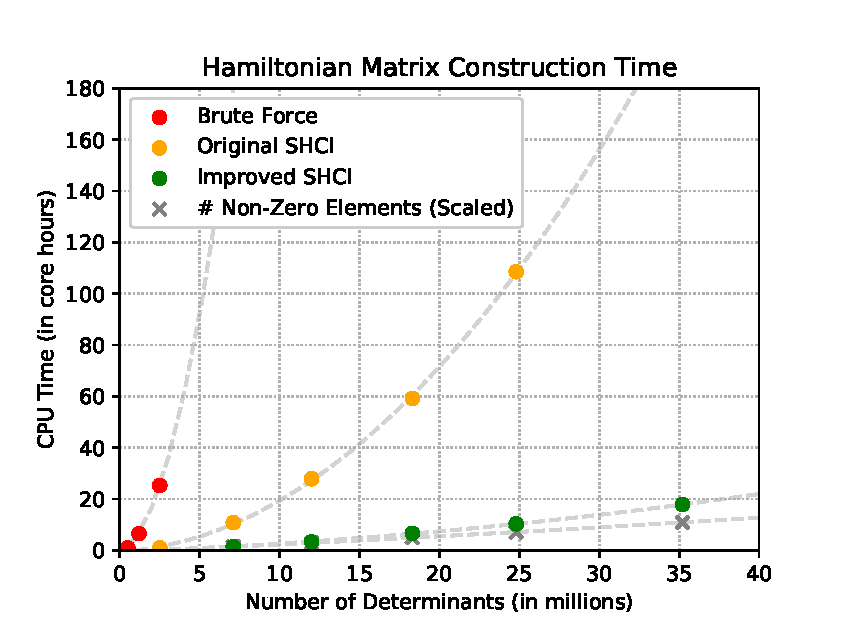
\includegraphics[width=\linewidth]{speedup/speedup.eps}
  \caption{Hamiltonian matrix construction time for a copper atom in a cc-pVTZ basis. Hamiltonian construction is the performance bottleneck in the variational stage.
%This figure shows that Fast SHCI's new Hamiltonian construction algorithm is an order of magnitude faster than SHCI and several orders of magnitude faster than brute force (loop over each pair of determinants).}
Hamiltonian construction in our improved SHCI algorithm is an order of magnitude faster than in
our original SHCI algorithm, and several orders of magnitude faster than the faster of the two brute force
approaches (loop over each pair of determinants).
Also shown is the number of nonzero elements in the Hamiltonian, scaled so that the first point coincides with
the first point of the improved SHCI CPU time.}
  \label{fig:ham}
\end{figure}

In Fig~\ref{fig:ham}, we use a copper atom~\footnote{We employ the Trail-Needs pseudopotential~\cite{TraNee-JCP-15},
but the conclusions of this paper would be the same for an all-electron calculation.}
in the cc-pVTZ basis to compare the improved SHCI algorithm to the original SHCI algorithm,
and to the brute force algorithm where we loop over each pair of determinants.
The improved algorithm
is about an order of magnitude faster than the original SHCI for medium size calculations.
For large calculations, e.g. the Cr$_2$ calculation described in Section~\ref{results}
where we use billions of variational determinants, the speedup is even greater.

\section{3-step Perturbation Energy}
%\subsection{3-step Perturbation Energy}
\label{multi}

As described in Section~\ref{overview}, our original SHCI algorithm~\cite{ShaHolJeaAlaUmr-JCTC-17} solves the memory bottleneck problem of SCI+PT methods
by introducing a semistochastic algorithm for computing the perturbative correction to the energy.
In Section~\ref{overview} we have emphasized that the
% efficiency of the calculation can dramatically improved
statistical error can be dramatically reduced
by decreasing the value of $\epsilon_2^{\rm dtm}$ in Eq.~\ref{eq:semistoch_PT}, and by increasing the size of the stochastic samples, $N_d$ in Eq.~\ref{eq:stoch_PT}.
This occurs for two reasons:
First, by using a smaller value of $\epsilon_{2} ^{\rm dtm}$ a larger fraction of the perturbative energy is computed deterministically
and so the portion being evaluated stochastically has smaller expectation value and smaller fluctuations.
Second, for a given total number of samples, the statistical error is smaller for a small number of large samples,
than for a large number of small samples, because the number of sampled contributions to the energy correction is a quadratic function
of the number of sampled variational determinants.
%{\color{red} Sandeep, I added the above explanations because you pointed out that most people would think that only the total
%number of samples would be relevant.  We can leave it here if you like, but it is probably not really necessary, because it is already
%there in the review section. -- Cyrus}

However, decreasing $\epsilon_2^{\rm dtm}$ or increasing $N_d$ can quickly lead to calculations that require very large memory
making the calculations impractical even on large computers. In this situation, one is left with no choice but to run relatively
inefficient calculations with larger $\epsilon_2^{\rm dtm}$ and smaller $N_d$.
For example, in Table~\ref{tab:pt} rows 3 and 4 show a comparison of the total CPU time of the perturbation stage
for a copper atom in a cc-pVTZ basis on a machine with large memory versus on a machine with small memory.
% {\color{red} can you specify epsilond and N in the table as well? -- Sandeep}.
% {\color{blue} I intentionally exclude the details so that people won't misinterpret the timing and use that for comparison as the Berkeley paper did.  -- Junhao}\\
% {\color{red} Yes, those kind of paper are terrible because people start writing defensively, like we are doing. But I wonder if misinterpreting things like the Berkeley paper will become more difficult if we give more details. For example if we say that the deterministic calculation took xx cpu seconds to get xx accuracy, then to prove that their code is better, they will probably have to do more of an apples to apples comparison. With the current data they might try to get a 1e-8 accuracy and then multiply our timings with $100^2$.  -- Sandeep}.
When we decrease the memory by a factor of four, the total CPU time of the original SHCI algorithm increases by almost a factor of 8.

%For a given statistical error there is a choice for $\epsilon_2^{\rm dtm}$ and the size of each stochastic sample, $N_d$,
%in Eqs.~\ref{eq:semistoch_PT} and \ref{eq:stoch_PT} that minimizes the computer time.
%We define a computer that does not permit the use of these optimal values to be a memory-constrained environment.
%In memory constrained cases, the product of the size of the stochastic sample and number of samples is much larger than on a system with sufficient memory.
%From our empirical experience, this occurs when the memory required to store the entire perturbative space is more than a few hundred times larger than the available system memory.
%Unfortunately, most interesting systems have huge Hilbert spaces, and therefore sufficiently large perturbative spaces
%that even large memory computer clusters become memory constrained environments, leading to a performance bottleneck.

\begin{table}[h]
  \begin{tabular}{| c | c | c | c |}
  \hline
  Method & Memory & \begin{tabular}{@{}c@{}}CPU Time \\ (core hours)\end{tabular} & Error ($\mu$Ha) \\
  \hline\hline
  HCI (deterministic) & 3TB & 145.0 & 0 \\
  \hline
  \multirow{2}{*}{Original SHCI} 
  & 32GB & 116.6 & 10 \\
  \cline{2-4}
  & 128GB & 14.5 & 10 \\
  \hline
  \multirow{3}{*}{Improved SHCI}
   & 32GB & 4.2 & 9 \\
  \cline{2-4}
   & 128GB & 3.7 & 9 \\
  \cline{2-4}
   & 128GB & 5.9 & 1.8 \\
  \hline
  \end{tabular}
    \caption{
    % {\color{red} Can you include the sample size, number of samples and the cost/sample for atleast the original algorithm (preferably for all). The cost/sample hopefully scales linearly with the size of sample. The data in this table can be used to emphasize that even if the product sample size X the number of samples (which should be proportional to the cpu cost) is the same, the calculation with larger sample size will be more efficient. This is quite non-intuitive and is the main motivation for developing the new algorithm -- Sandeep.}\\
    Computational cost of perturbative correction for a copper atom in a cc-pVTZ basis.
    The variational space has 19 million determinants for $\epsilon_1=5\times10^{-5}$~Ha and the perturbative space has 35 billion determinants for $\epsilon_2=10^{-7}$~Ha.
    HCI uses the deterministic perturbation of Ref.~\onlinecite{HolTubUmr-JCTC-16}.
    SHCI uses the 2-step semistochastic perturbation algorithm of Ref.~\onlinecite{ShaHolJeaAlaUmr-JCTC-17}.
    Improved SHCI introduces the 3-step batch perturbation that significantly improves the efficiency of SHCI, especially for memory constrained cases.
    The timings for the 32GB machine are obtained by running on the same 128GB large memory machine but intentionally tuning the parameters so that the memory usage is kept below 32GB throughout the run.
    We also provide the timing to reach a 1.8~$\mu$Ha uncertainty to illustrate that our statistical error goes down much faster than $1/\sqrt{T}$ since we use smaller $\epsilon^{\rm dtm}_2$ and $\epsilon^{\rm psto}_2$ values for smaller target errors.
}
  \label{tab:pt}
\end{table}

For a given target error, assuming we have infinite computer memory, there is an optimal choice of $\epsilon_2^{\rm dtm}$ and $N_d$
for reaching that target error using the least computer time.
%Our improved algorithm is designed to allow us to always use parameters such that the efficiency of the calculation does not
%depend strongly on the available computer memory.
Our improved algorithm is designed to have an efficiency that depends only weakly on the available computer memory.
It is always more efficient than the original algorithm, especially when running on computers with small memory, in which case the
gain in efficiency can be orders of magnitude.
To achieve that we replace the original 2-step SHCI algorithm with a 3-step algorithm.
In each of the three steps, the perturbative determinants are divided into batches using a hash function~\cite{Jen-Hash-97, Boost-2012},
and the energy correction is computed either by adding, in succession, the contribution from each batch,
or by estimating their sum by evaluating
% sampling
% $-$ without replacement $-$
% (without replacement)
only a subset of these batches.
Hence our improved SHCI algorithm has the following 3 steps:
\begin{enumerate}
\item A deterministic step with cutoff $\epsilon_2^{\rm dtm} (< \epsilon_1)$, wherein all the perturbative batches are summed over.
\item A ``pseudostochastic" step, with cutoff $\epsilon_2^{\rm psto} (< \epsilon_2^{\rm dtm})$, wherein typically only a small fraction of the perturbative batches
need be summed over to achieve an error much smaller than the target error.
\item A stochastic step, with cutoff $\epsilon_2 (<\epsilon_2^{\rm psto}) $, wherein a few stochastic samples of variational determinants,
each consisting of $N_d$ determinants, are sampled using Eq.~\ref{sampling_prob} and only one of the
perturbative batches is randomly selected per variational sample.
\end{enumerate}
%The cutoffs get progressively smaller, i.e., $\epsilon_1 > \epsilon_2^{\rm dtm} > \epsilon_2^{\rm psto} > \epsilon_2$.
The choice of these parameters depends on the system and the desired statistical error, but
reaonable choices for a target error around $10^{-5}$~Ha are  $\epsilon_2^{\rm dtm} = \max(\epsilon_{1}/50,10^{-6}$~Ha),
$\epsilon_2^{\rm psto} = \max(\epsilon_{1}/500,10^{-7}$~Ha), and,
$\epsilon_2 = \epsilon_{1}/10^6$.
%Of course, for small systems we can use smaller values of $\epsilon_2^{\rm dtm}$ and $\epsilon_2^{\rm psto}$, and employ
%just the first two, or even just the first step of the perturbative calculation.
We next describe each of the 3 steps in detail.

%Sandeep:
%Our improved algorithm is designed to allow us to use smaller $\epsilon_2^{\rm dtm}$ and larger values of $N_d$
%without increasing the memory requirement of the calculation.
%The key ingredient of the new algorithm is that
%now we partition the determinants in the $\P$ space into batches using a hash function~\cite{Jen-Hash-97, Boost-2012},
%and one can then use the fact that the total perturbation correction is equal to the sum of contributions from each batch.
%To make effective use of the batches we modify the original 2-step SHCI algorithm into one that makes use of the the following 3-steps
%\begin{itemize}
%\item first, a series of deterministic steps are performed with a cutoff $\epsilon_2^{\rm dtm}$, where in each step the contribution from only a single batch is evaluated and is subsequently accumulated
%\item second, a Monte Carlo summation of the contribution from all the batches is calculated by performing several iterations in which the perturbative contribution of a randomly selected batch (without repeats) is calculated with with a cutoff $\epsilon_2^{\rm psto}$ ($< \epsilon_2^{\rm dtm}$), and,
%\item third, a stochastic step, with cutoff $\epsilon_2$ ($<\epsilon_2^{\rm psto}$) is performed where a sample of $N_d$ variational determinants and also a batch of perturbative determinants is randomly selected.
%\end{itemize}

%Junhao:
%% We don't do larger dtm or sto runs. we do optimal runs.
%For a given target error, assuming we have infinite amount of memory, there is a set of optimal meta parameters for reaching that target error in the shortest time.
%Our improved algorithm is initially designed to allow us to always use optimal values of $\epsilon_2^{\rm dtm}$ and $N_d$ regardless of the memory available.
%To achieve that, we partition the determinants in the $\P$ space into batches using a hash function~\cite{Jen-Hash-97, Boost-2012}, and we can then use the fact that the total perturbation correction is equal to the sum of contribution from each batch.
%
%While doing the batch calculations, we find that with a high-quality hash function, the contribution from different batches are almost the same.
%Hence, we can evaluate just a few batches and use them to estimate the total contribution from all the batches.
%
%Based on these ideas and findings, we develop the 3-step batch perturbation method.

%% In addition to the original 2-step algorithm, we introduce a new pseudo stochastic step between them, and we apply the batch idea to all of the 3 steps.
%% We describe each of the 3 steps in detail.
%% To make effective use of the batches we modify the original 2-step SHCI algorithm into one that makes use of the the following 3-steps
%% \begin{itemize}
%% \item First, a series of deterministic steps are performed with a cutoff $\epsilon_2^{\rm dtm}$, where in each step the contribution from only a single batch is evaluated and is subsequently accumulated
%% \item Second, a Monte Carlo summation of the contribution from all the batches is calculated by performing several iterations in which the perturbative contribution of a randomly selected batch (without repeats) is calculated with with a cutoff $\epsilon_2^{\rm psto}$ ($< \epsilon_2^{\rm dtm}$), and,
%% \item Third, a stochastic step, with cutoff $\epsilon_2$ ($<\epsilon_2^{\rm psto}$) is performed where a sample of $N_d$ variational determinants and also a batch of perturbative determinants is randomly selected.
%% \end{itemize}

The first step is a deterministic step similar to the original SHCI's deterministic step,
% except that we use a smaller $\epsilon_2^{\rm dtm}$
except that when there is not enough memory to afford the
% optimal
chosen $\epsilon_2^{\rm dtm}$, we divide the perturbative space into batches according to the hash value of the perturbative determinants and evaluate their contributions batch by batch.
This deterministic step has the effect of greatly reducing the computational effort required to obtain a given statistical
error in the subsequent steps.
% We calculate the perturbation correction one batch at a time.
When there is not enough memory to perform the original deterministic run with the
%optimal choice of
chosen $\epsilon_2^{\rm dtm}$, we divide the hash value space into several batches, and for each batch
we calculate its contribution from only the perturbative determinants whose hash value belongs to that batch.
The total deterministic correction is simply the sum of the corrections from all the batches
\beq
%$$\Delta E_{2}^{(d)} \left(\epsilon \right) = \sum_ {B} \sum_{D_{a}} \frac{\left(\sum_{D_{i} \in \V, \left|H_{a i} c_{i}\right| \ge \epsilon_{2}, h(D_a)\in B} H_{a i} c_{i}\right) ^{2}}{E_{V} - H_{a a}}$$
%$$\Delta E_{2} \left(\epsilon^{\rm det} \right) = \sum_{B} \sum_{D_{a} \in \P, h(D_a)\in B} \frac{\left(\sum^{(\epsilon_{2}^{\rm det})}_{D_{i} \in \V} H_{a i} c_{i}\right) ^{2}}{E_{V} - H_{a a}}$$
\Delta E_{2} \left(\epsilon_2^{\rm dtm} \right) = \sum_{B} \sum_{\substack{D_{a} \in \P \\ h(D_a)\in B}} \frac{\left(\sum^{(\epsilon_2^{\rm dtm})}_{D_{i} \in \V} H_{a i} c_{i}\right) ^{2}}{E_{V} - H_{a a}}
\eeq
where $h(D)$ is the hash function and $B$ is the hash value space for a batch.
This method solves the memory bottleneck in a different way than the original SHCI algorithm.
We could do the full calculation in this way, i.e., use a very small value for $\epsilon_2^{\rm dtm}$,
but it is much more efficient to only evaluate the large contributions here and leave the huge number of small contributions to the later stochastic steps.
Typically, we choose $\epsilon_2^{\rm dtm} = \max(\epsilon_{1}/50, 10^{-6}$~Ha) for a target error of $10^{-5}$~Ha.
%The threshold $10^{-6}$ depends on the target statistic error we want.
%From our experience, $10^{-6}$ is usually around the optimal choice for a target error of $10^{-5}$~mHa.
% but since it requires regenerating the perturbative space for each batch, this is not
% efficient when the number of batches becomes large.
%To get better performance, we usually use
%% $\epsilon_2^{\rm dtm} \approx \epsilon_{1}/50$ for this step
%a modest number of batches,
%and leave the perturbative contributions for smaller $\epsilon$ to later steps.
%Even though we can use lots of batches to do a deterministic epsilon_small calculation directly,
%we can do it orders of magnitude faster by doing an epsilon_big first to get most of the correction
%and then get the additional small correction for epsilon_small by evaluating just a small subset of all the batches.
%Typically, for large calculations, 1 out of 100 batch is enough to get a total statistical error < 0.01 mHa
%because the hash function is quite uniform and the remaining correction is small.
% Instead, we can do it orders of magnitude faster by using a large value of $\epsilon_2^{\rm dtm}$ (say $\epsilon_2^{\rm dtm} \approx \epsilon_{1}/50$)
% and then getting the remaining small correction for small $\epsilon_2$ in the pseudo-stochastic and stochastic steps
% using just a small subset of the batches.

%{\color{red} The determinisitc with batches is clear to me, but the following two are not entirely clear. for exmaple you are sampling the variational determinants and the PT determinants as well and more words are needed to describe how exactly this is done. Again I think if it is possible provide a pseudo code or a figure then it will make things much easier to understand.}
The second step is a pseudo stochastic step.
It is similar to the deterministic step, except for the following differences: 
a) we use an $\epsilon_2^{\rm psto}$ much smaller than $\epsilon_2^{\rm dtm}$ as the selection criterion,
b) we divide the perturbative space into as many batches as is needed in order for one batch to fit in memory,
with the constraint that there are at least 16 batches,
c) we use the corrections from the perturbative determinants in a small subset of the batches (often one is enough)
to estimate the total correction from all the perturbative determinants, as well as its standard error.
Looping over batches, for each batch, we calculate the correction from each unique perturbative determinant in that batch.
We accumulate the number of unique determinants, the sum and the sum of squares of the corrections from these determinants.
At the end of each batch iteration, we calculate the mean and standard deviation of the corrections from all the
evaluated perturbative determinants and use these to estimate the total correction from all the perturbative determinants.
Note that the standard deviation of the total correction is the standard deviation of the sum of only the unevaluated determinants.
%If we process all the batches, the second step becomes a deterministic calculation, which has zero uncertainty.
If we process all the batches, the pseudo stochastic step becomes deterministic and has zero standard deviation.
%At the end of each batch iteration, we scale these three values by the ratio between the remaining number of batches and the number of evaluated batches to estimate these three values for all the perturbative determinants, which
%give us both the total correction and the standard deviation of the total correction.
% We calculate the energy correction from the batch and the variance of the energy correction from the batch. (I don't do that for each batch)
% We then scale these by the number of remaining batches to estimate total energy correction and its standard deviation. (scaled by the ratio)
When the standard deviation of the total correction is smaller than 40\% of the target error, we exit the loop over batches.
%However, since we have a good hash function, a single batch is often enough to reach a statistical error below that threshold
However, a single batch is often sufficient to reach a statistical error below that threshold,
and we have never found a case where we need to evaluate more than 10\% of the batches.
Typically, for a target statistical error of $10^{-5}$~Ha, we choose $\epsilon_2^{\rm psto} = \max(\epsilon_{1}/500, 10^{-7}$~Ha).

% we estimate the total correction and its standard deviation based on the assumption that the sum and the standard deviation of the corrections from each of the remaining batches are the same as the averages of the evaluated batches.
% This assumption is based on our numerous empirical evidence that both the sum and standard deviation almost do not change between batches.

%($\epsilon_2^{\rm psto} < \epsilon_2^{\rm dtm}$),
% and the batch loop is exited
% when the number of batches is greater than 5 and the uncertainty from the processed batches
% is much smaller than the target error.
%In practice we use $\epsilon_2^{\rm psto} \approx \epsilon_{1}/500$ and exit the loop when the uncertainty
% drops below 20\% of the target error.
% Typically only a small fraction of the batches are needed in this step.{\color{red} How are you averaging? Does the fact that you don't allow any repeats make it complicated?}

The third step is a stochastic step that is similar to the stochastic step of the original SHCI algorithm, except that instead of keeping all the perturbative determinants
that satisfy the $\epsilon_2$ criterion we keep only one randomly selected batch out of several.
The available computer memory constrains the number of perturbative determinants, and one can obtain the same number sampling a certain
number of variational determinants and all the perturbative determinants that satisfy the $\epsilon_2$ criterion (the original SHCI algorithm),
or, by using a larger number of variational determinants and selecting just one batch of the perturbative determinants.
The latter allows us to use much larger variational samples.
Using larger variational samples is advantageous because we find that the additional fluctuations
%due to sampling the perturbative determinants is much smaller than the additional fluctuations due to having smaller variational samples.
due to sampling the perturbative determinants is much smaller than the reduction in the fluctuations due to having larger variational samples.
Typically, we use $\epsilon_2 = 10^{-6} \epsilon_{1}$.  Since the smallest $\epsilon_{1}$ that we use is typically around $10^{-5}$~Ha,
this value is in fact much smaller than is needed to ensure that the perturbative correction is fully converged.
For a statistical error of $10^{-5}$~Ha, 128 batches is usually a good choice to start with.
The size of the variational sample is chosen so that a single perturbative batch fits in the available memory.
We use a minimum of 10 samples in our stochastic step in order to get a meaningful estimate of the uncertainty.
On large memory machines, we often achieve a much smaller statistical error than the target with 10 samples.
In that case, we can decrease the size of the variational sample in later runs for similar systems.
% We also have put in our implementation the ability to use the maximum number of samples allowed for a given percentage of the memory.
% After we do a quick run, we can adjust the number of samples accordingly to make the number of iterations required to reach the target error roughly 10.
% We use 10 as the minimal number of iterations in our stochastic step so that we can get a meaningful estimation of the uncertainty.


%{\color{red} How are you using correlated samples here? Are the batch size at each of the three levels the same? I think it needs a few words.}
% We don't use correlated samples.

In Table~\ref{tab:pt}, the last four rows compare the original SHCI to the improved version with 3-step batch perturbation.
In the memory-constrained case, the improved SHCI runs more than an order of magnitude faster than the original SHCI.
Even when memory is abundant, the improved SHCI is still a few times faster.

The main reasons that the improved SHCI is much faster are:
%(1) It computes a larger fraction of the perturbative correction in the deterministic step, and it uses much larger samples
(1) It computes a larger fraction of the perturbative correction in the deterministic step.
(2) A small fraction of the batches in the pseudo stochastic step is usually sufficient to give an accurate estimate of the total correction.
(3) It uses much larger samples of variational determinants in the stochastic runs.

We now comment on a couple of aspects of our algorithm that are not obvious.
% In the pseudo stochastic step, we estimate the batch-to-batch fluctuations from just the fluctuations within a batch.
% This relies on having a sufficiently good hash map and the fact that we have a very large number of perturbative determinants
% in each batch (sometimes a billion or more).
% Note that since we are using all the variational determinants in this step, the fluctuations come just from the perturbative
% determinants.
In the pseudo stochastic step, we estimate the fluctuations of the unevaluated perturbative determinants from the fluctuation of the evaluated perturbative determinants.
This relies on having a sufficiently uniform hash function.
% and the fact that we have a very large number of perturbative determinants
% in each batch (sometimes a billion or more). % not needed.
Note that since we are using all the variational determinants in this step,
the fluctuations come just from the perturbative determinants.
In contrast, in the stochastic step, the fluctuations come both from the choice of variational determinants and the choice of batches.
In that case, one cannot simply use the standard deviation of the corrections from the evaluated perturbative determinants to estimate the standard deviation of the total correction.
% In that case, one cannot use the intra-batch fluctuations to estimate the inter-batch fluctuations.  
So, in the stochastic step we use a minimum of 10 samples, calculate the correction from each of these samples,
and use standard deviation of these sample corrections to estimate the standard deviation of the total correction.

Another point to note is that the use of batches carries a small computational overhead of having to regenerate the
perturbative determinants for each batch.  Using our method, generating determinants is sufficiently fast that the
increase in computational cost would be substantial only if this is done many times.  If we employed a purely
deterministic algorithm, the number of batches would be very large, but with our 3-step semistochastic algorithm
the number of batches actually computed is sufficiently small in each of the three steps that there is never a large computational overhead.

Finally, we comment on two other algorithms that have been recently been proposed for calculating the perturbative correction.
%We note that another very efficient semistochastic algorithm for calculating the perturbative correction has been proposed
First, another very efficient semistochastic algorithm has been proposed
by Garniron et al.~\cite{GarSceLooCaf-JCP-17}.  However, that algorithm has, for each perturbative determinant, a loop over the variational determinants to find those that are connected.  For the very large number of variational determinants that we employ
here (up to $2 \times 10^9$) this is less efficient than our algorithm.
To avoid confusion, we should mention that the reason that their energy for Cr$_2$ is very different from ours is
that they used a nonrelativistic Hamiltonian.
Second, another algorithm that uses batches of perturbative determinants to overcome the memory bottleneck has been proposed
very recently~\cite{TubLevHaiHeaWha-ARX-18}.
It is an efficient deterministic algorithm for memory constrained environments,
but for a reasonable statistical error tolerance, e.g., $10^{-5}$~Ha,
a semistochastic approach is usually much faster, as we can see from Table~\ref{tab:pt}.
Also, in our Cr$_2$ calculation, we stochastically estimate the perturbative correction from at least trillions of perturbative determinants,
for $\epsilon_2=3\times10^{-12}$, which probably involves quadrillions of contributions, which is infeasible with a deterministic algorithm.
% The largest calculations in that paper use only $2 \times 10^6$ variational determinants, three orders of magnitude
% less than our largest ones.


\section{Key Data Structures}
\label{key}
%In this section, we discuss three key data structures in our SHCI implementation: the determinants, the distributed Hamiltonian matrix, and the distributed partial sums.
In this section, we discuss three key data structures used to store the determinants, the distributed Hamiltonian matrix, and,
the distributed partial sums in the perturbative stage of the calculation.

\subsection{Determinants}
\label{{sec:det}}
%We use two different representations of determinants in different parts of our implementation.
%
%When storing and accessing determinants locally in memory, we use bit-packing with 64-bit unsigned integers.
%Each bit represents an orbital.
%Hence, the n-th orbital is represented by the  \lstinline{(n | 63)}-th bit of the \lstinline{(n >> 6)}-th integer, where ``\lstinline{|}'' is the bitwise ``or'' and ``\lstinline{>>}'' is the bitwise right shift.
%
%When we transfer the determinants to other nodes or save them to the file system, we use base-128 varints~\cite{stuart2012encoding} to compress the integers before pushing them to the network or file stream.
%This compression reduces the network traffic and the sizes of the wavefunction files significantly, especially for large basis sets.

We use two different representations of determinants.
For storing and accessing determinants locally in memory, we use arrays of bit-packed 64-bit unsigned integers.
Each bit represents a spin-orbital.
%Using the ridiculous {\color{red} maybe don't say this?} C++ convention that indices start at zero, the n-th orbital is represented by the \lstinline{(n | 63)}-th bit of
%the \lstinline{(n / 64)}-th integer, where ``\lstinline{|}'' is the bitwise ``or'' and ``\lstinline{/}'' is integer division.
%{\color{red} Is the bitwise ``or'' part correct? It seems like this sentence detracts more than it adds, and should be removed.}
The n-th orbital is represented by the (n mod 64)-th bit of
the \lstinline{(n / 64)}-th integer, where ``\lstinline{/}'' means integer (Euclidean) division and the counting starts from zero.
% If count from one, it is going to be (((n-1) mod 64) + 1)-th bit of the ((n-1)/64+1)-th integer, which is more confusing and is different from the implementation.
(n mod 64) can be implemented as \lstinline{(n & 63)}, and \lstinline{(n / 64)} can be implemented as \lstinline{(n >> 6)},
where ``\lstinline{&}'' is the bitwise ``and'' and ``\lstinline{>>}'' is the bitwise right shift.
% {\color{red} \lstinline{(n >> 6)} (MJO - is 6 correct? Or should it be 64? 6 seems odd}
Both operations cost only one clock cycle on modern CPUs.

For transferring the determinants to other nodes or saving them to disk, we use base-128 variable-length integers
%(VarInts)~\cite{stuart2012encoding} to compress the integers.
(VarInts)~\cite{StuFer-Protobuf-12} to compress the 64-bit integers.
VarInts take only a few binary operations to compute and reduce the memory footprint by up to 87.5\% for small integers, which reduces the network traffic and the size of the wavefunction files considerably, especially for large basis sets.

\subsection{Hamiltonian Matrix}

We store only the upper triangle of the Hamiltonian matrix.
The rows are distributed to each node in a round-robin fashion: the first row goes to the first node, the second row goes to the second node,
and when we reach the end of the node array, we loop back and start from the first node again.
Each row is a sparse vector, represented by two arrays, one stores the indices of the nonzero elements and the other stores the values.


During the matrix-vector multiplication, each node will apply its own portion of the Hamiltonian to the vector to get a partial resulting vector.
The partial results are then merged together using a binomial tree reduction.
The work on each node is distributed to the cores with dynamic load balancing.
To save space, we store only one copy of the partial resulting vector on each node and each thread updates that vector with hardware atomic operations.
In addition, we cache the diagonal of the matrix on each node to speed up the Davidson diagonalization~\cite{Dav-CPC-89}.

\subsection{Partial Sums}
%In the perturbation stage, we need to loop through all the variational determinants $D_i$ and accumulate $H_{ai}c_{i}$ to get the partial sum $\sum H_{ai}c_{i}$ for each perturbative determinant $D_a$.
%To store this mapping relationship from $D_a$ to $\sum H_{ai}c_{i}$, we use a distributed hash table.
%
%The choice of using a hash table versus using a sorted array is based on the number of determinants that we are dealing with.
%The time complexity inserting one element to the hash table is ${\cal O}(1)$, while for a sorted array it is ${\cal O}(\log(n))$.
%We use up to 274 billion determinants in our deterministic perturbation.
%For calculations at this scale, the prefactor from using hash tables becomes negligible, and the contribution from the $\log(n)$ becomes enormous.
%
%The distributed hash table is based on lock-free linear-probing concurrent hash tables.
%Linear-probing has better efficiency than chaining for intensive parallel insertion, and the lock-free implementation allows all the threads operate at their full speed.
%On each node, we have $n$ of these concurrent hash tables, where $n$ the total number of nodes.
%One of them stores the entries belong to this node, and other $(n-1)$ tables store the entries belong to other nodes pending synchronization.

In the perturbative stage, we loop over all the variational determinants $\{D_i\}$ to compute the partial sum $\sum_i H_{ai}c_{i}$
for each perturbative determinant $D_a$.
The map from $D_a$ to $\sum_i H_{ai}c_{i}$, is stored in a distributed hash table.
%The choice of using a hash table versus using a sorted array is based on the number of determinants that we are dealing with.
This choice is dictated by the enormous number of perturbative determinants we employ.
The time complexity of inserting one element into the hash table is ${\cal O}(1)$, while for a sorted array it is ${\cal O}(\log(n))$.
For large calculations, the prefactor from using hash tables is small compared to the $\log(n)$ cost from using a sorted array.

%{\color{red} The following paragraph is not entirely clear to me.}
The distributed hash table is based on lock-free open-addressing linear-probing concurrent hash tables specifically designed
for intensive commutative insertion and update operations.
%, which is exactly the case for accumulating the partial sums.
The linear-probing technique for conflict resolution has better efficiency than separate chaining during parallel insertion,
and the lock-free implementation allows all the threads to almost always operate at their full speed.

On each node, we have $n$ of these concurrent hash tables, where $n$ is the number of nodes.
One of them stores the entries belonging to this node, and the other $(n-1)$ tables store the entries belonging to other nodes pending synchronization.
Each concurrent hash table is implemented as lots of segments (at least four times the number of hardware threads) and each segment can be modified by only one thread at a time.
When a thread wants to insert or update a (key, value) pair, it first checks whether the segment that the key belongs to is being used by other threads.
If the segment is being used, the thread will insert or update the entry to a thread-local hash table, which will be merged to the main table later periodically.
We can do this because the insertion and the update operations of the partial sums are commutative.
Hence, each insertion and update is guaranteed to finish within ${\cal O}(1)$ time without getting blocked, even for perturbative determinants with lots of connections to the reference determinants.
The inter-node synchronization also runs periodically so that most of the perturbative determinants will have only one copy during the entire run on the entire cluster, except for those with lots of connections to the reference determinants.
% In the end when all the threads are done with the update, the data belongs to other nodes will be compressed with the algorithm in {sec:det} and sent to the corresponding nodes.

\section{Parallelization}
\label{para}

All the critical parts of SHCI are parallelized with MPI+OpenMP.
This section describes the parallelization and the scalability of each part.

When finding the connected determinants, performing the matrix-vector multiplication during the diagonalization,
and constructing the Hamiltonian matrix from the auxiliary arrays, we use the round-robin scheme to distribute the load across the nodes
and use dynamic load balancing for all the cores on the same node.

%We parallelize the construction of the $\alpha$ singles and $\beta$ singles arrays on each node, which is the bottleneck of constructing the auxiliary arrays.
%To parallelize this part, we first updated $\alpha$ and $\beta$ array which contains the $\alpha$ and $\beta$ that belong to the new determinants found in the current variational iteration.
%For each of them, we initialize a singles array and a lock to ensure exclusive modification.
%Then, we do the following for each $\alpha$ in parallel:
%We go through the $\alpha-1$ array of that $\alpha$ to find all the $\alpha^\prime$s that are one excitation away.
%We lock and append $\alpha^\prime$ to the single array of $\alpha$.
%Similarly, we lock and append $\alpha$ to the single array of $\alpha^\prime$.
%When both $\alpha$ and $\alpha^\prime$ are in the updated $\alpha$ array, only the smaller of the two do the update.

We parallelize the construction of the $\alpha$-singles and $\beta$-singles arrays on each node, which is the most time-consuming part of constructing the auxiliary arrays.
%We first update the $\alpha$ and $\beta$ arrays to add in the $\alpha$ and $\beta$ strings of the new determinants found in the current variational iteration,
%if the $\alpha$ and $\beta$ strings were not already present.
%Then we update the $\alpha-1$ and $\beta-1$ arrays to include the $\alpha-1$, $\beta-1$, $\alpha$, $\beta$ strings that were not already present.
%Then we construct $\alpha$-singles and $\beta$-singles arrays in parallel on each node:
For each entry of $\veciaa$ and $\vecibb$, we initialize a lock to ensure exclusive modification.
%Then, we do the following for each $\alpha$ in parallel:
%We go through the $\alpha-1$ arrays of that $\alpha$ to find all the $\alpha^\prime$s that are one excitation away.
We loop over all the $\vecia({\alpha^{(-1)}})$ arrays and for each ($\ia$, $\ja$) pair (which are one excitation away) inside a particular $\vecia({\alpha^{(-1)}})$ array,
we lock and append $\ja$ to $\veciaa{(\ia)}$, and
we lock and append $\ia$ to $\veciaa{(\ja)}$.
When both $\ia$ and $\ja$ occur only in the new determinants, the smaller of the two does both appends.

In Figs.~\ref{fig:paravar} and \ref{fig:parapt}, we demonstrate the parallel scalability of our SHCI implementation
when applied to a copper atom in a cc-pVTZ basis. We use up to 16 nodes, and each node has 6 cores.

For the variational part, our implementation scales almost linearly up to 4 nodes.
% we see a diminishing return with respect to the number of nodes.
% This is most likely to be caused by the inter-rack bandwidth limit, which is shared with lots of other jobs.
% We can see that for up to 4 nodes, our code scales almost linearly. 
% After eight nodes, there is still only a slight deviation from the perfect scaling.
At 16 nodes we have 75\% parallel efficiency.
% , which should reflect the true scaling in an ideal environment.
% Then, there is a significant drop in the performance from 8 nodes, which we believe it is mainly because the job scheduler was not able to put all the eight nodes on one rack and decided to put some of them on different racks.

For the perturbative stage, two major factors determine the speedup.
One is the additional communication associated with
shuffling perturbative determinants across the nodes, which increases with the number of nodes.
The other is the speedup from having more cores.
% Not memory anymore.
We can see from Fig.~\ref{fig:parapt} that from 1 to 4 nodes, the first factor dominates and there is significant deviation from ideal speedup.
Starting from 8 nodes, we have to shuffle almost all the perturbative determinants from the spawning node to the storage node that each determinant belongs to,
so there is little change in the first factor and the second factor starts to dominate, pushing the speedup curve upward and producing almost perfect scaling.
Note that in the original SHCI algorithm~\cite{ShaHolJeaAlaUmr-JCTC-17}, there is a superlinear speedup from using more nodes
because many stochastic samples are needed when running in a memory-constrained environment.
Here we have solved this problem with the 3-step batch perturbation, for which the number of stochastic samples
is almost always 10.  (We require a minimum of 10 samples in order to have a reasonable estimate of the stochastic error.)
Consequently, 
on memory constrained environments,
we achieve a few orders of magnitude speedup.
%compared to the original SHCI algorithm.
%for memory contrained environments where we need lots of samples orignally,
%we have a few orders of magnitude speedup compared to the original SHCI algorithm.

\begin{figure}[h]
  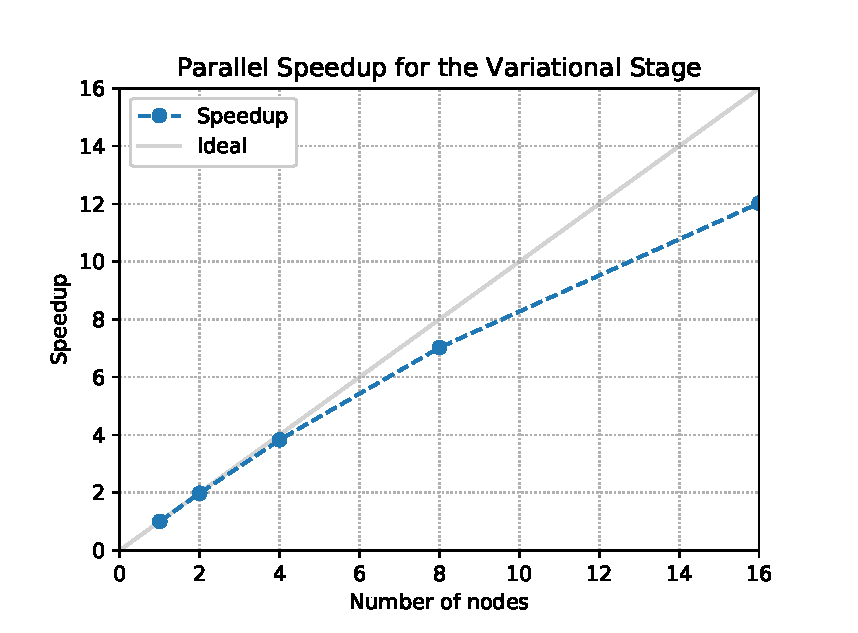
\includegraphics[width=\linewidth]{scalability/var}
  %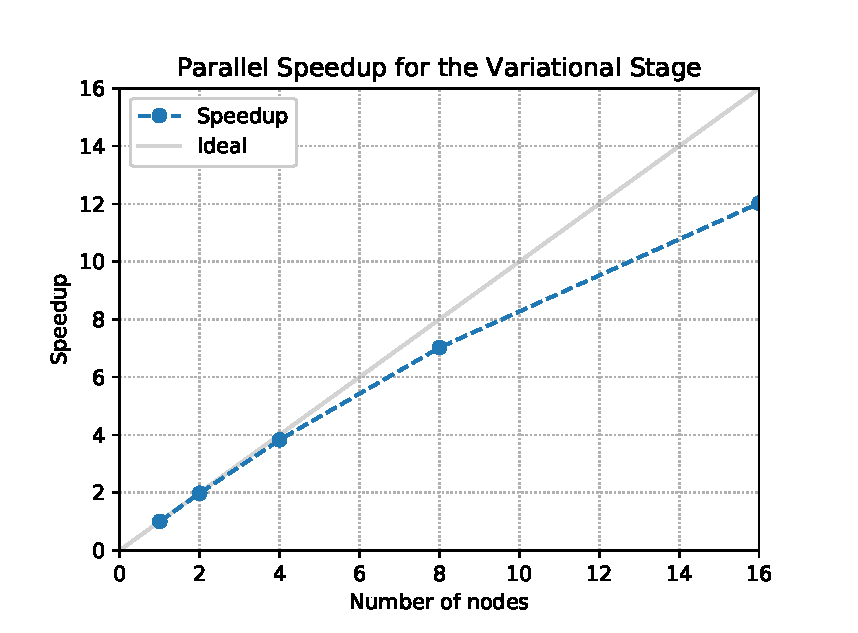
\includegraphics[width=\linewidth]{scalability/var.eps}
  \caption{Parallel speedup of the variational stage for a copper atom in a cc-pVTZ basis.
There is almost perfect scaling for up to 4 nodes and 75\% parallel efficiency at 16 nodes.
% Staring from 8 nodes, there is some significant drop in the performance, which we believe it is mainly because the job scheduler starts to place the nodes onto different racks.
}
  \label{fig:paravar}
\end{figure}
 
\begin{figure}[h]
  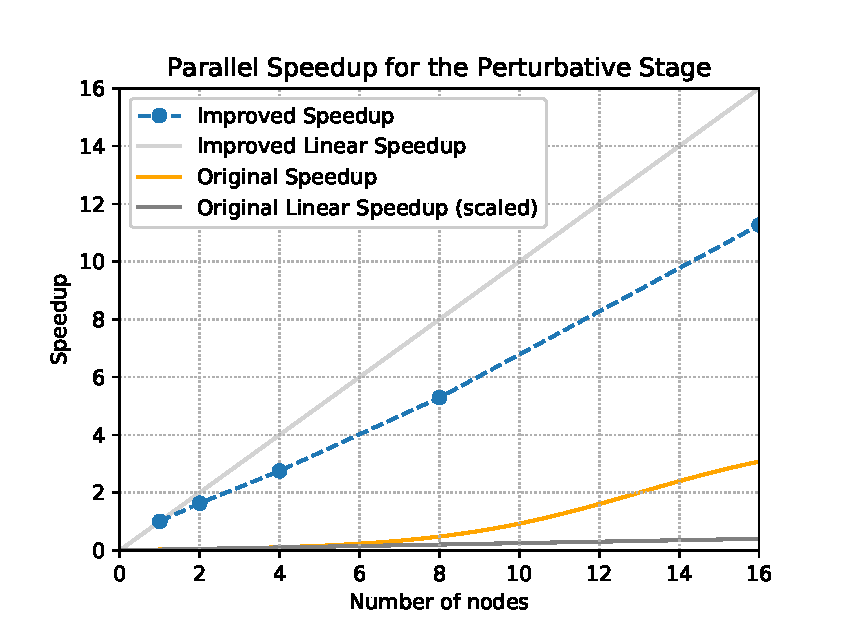
\includegraphics[width=\linewidth]{scalability/dtm.eps}
  \caption{
%{\color{red} my preference is to give cpu time on the y-axis and the guiding line to show ideal parallelization. -- Sandeep}\\
%{\color{blue} This would however have the downside of not being symmetrical with the speedup of the variational stage and
%also that linear scaling would now be an inverse power rather than linear.}\\
Parallel speedup for improved SHCI compared to the original SHCI for the perturbative stage of the
calculation for a copper atom in a cc-pVTZ basis.
From 1 node to 4 nodes, we see a significant deviation from linear speedup due to the additional communication from shuffling the perturbative determinants across nodes.
Starting from 8 nodes, the number of shuffles approaches a constant and we can see an almost linear speedup from using more processors.
The estimate of the speedup of the original SHCI is based on the assumption that the total memory of 10 nodes is enough to support
the optimal choice of $\epsilon_2^{\rm dtm}$ and $N_d$, in Eqs.~\ref{eq:semistoch_PT} and \ref{eq:stoch_PT}.
The ``Original" curves are scaled to reflect the relative speed of original SHCI algorithm to that of the improved algorithm.
}
  \label{fig:parapt}
\end{figure}

% \section{Fast SHCI}
% \label{Fast SHCI}
% For large calculations of SHCI, the two major performance bottlenecks are the Hamiltonian matrix construction and the stochastic perturbation.
% Fast SHCI makes significant improvements in both of them and can give a few orders of magnitude of overall speedup.

% Hamiltonian matrix construction becomes the major bottleneck in the variational stage due to the fact that SHCI solves the bottleneck with finding important determinants in SCI and can find millions of most important determinants in less than a core hour, but there is no efficient algorithm for generating such large Hamiltonian matrices that are associated with lots of determinants from high-order excitations yet.
% Fast SHCI addresses this issue and develop an efficient Hamiltonian matrix generation algorithm for large SCI calculations.

% The stochastic perturbation algorithm introduce by SHCI solves the memory bottleneck and can give a statistically unbiased perturbation result however large the perturbative space is.
% However, in memory constrained cases, SHCI may take thousands of stochastic iterations and uses a few orders of magnitude more core hours than needed when running on a large memory machine.
% Here ``large memory'' means large relative to the memory needed to store one-hundredth to one-tenth of the perturbative space determinants.
% Hence, for some interesting systems with huge Hilbert spaces, the perturbative spaces are so big that even the largest cluster on the earth would still be a memory constrained environment for these calculations.
% Fast SHCI introduces multistep batch perturbation, which also has a small memory footprint and has similar or faster speed than SHCI on large memory machines, but orders of magnitude faster than SHCI in memory constrained cases.

% The code that implements our algorithm can be found at \url{https://github.com/jl2922/shci}




\section{Results}
\label{results}

In this section, we apply SHCI to the chromium dimer, which is a challenging strongly-correlated system.
%We use a cc-pVDZ basis with active semi-core electrons.
We use a relativistic exact two-component (X2C) Hamiltonian, the cc-pVDZ-DK basis, and we correlate the valence and the semi-core electrons.
This gives an active space of (28e, 76o) and a Hilbert space of $5\times10^{29}$ determinants, which is far beyond the reach of full-CI.
We show how we obtain an accurate estimate of the full-CI energy in this large active space with our improved SHCI algorithm.

We use PySCF~\cite{SunCha_etal_PySCF-ComMolSci-18} to generate the molecular orbital integrals for orbitals that minimize the HCI variational
energy for $\epsilon_1=2\times 10^{-4}$~Ha, using the method of Ref.~\cite{SmiMusHolSha-JCTC-17}.
We perform SHCI with several $\epsilon_1$ values from $5\times10^{-5}$ to $3\times10^{-6}$~Ha.
The Hamiltonian matrix is constructed only once.
% The Hamiltonian matrix is stored in memory and so needs to be constructed only once.
%We keep the ratio between $\epsilon_2$ and $\epsilon_1$ to $10^{-6}$ and the target error for the stochastic perturbation to 0.01 mHa.
We use very small values of $\epsilon_2 = 10^{-6} \epsilon_1$  to ensure that the perturbative correction is exceedingly well converged,
and choose the target error for the stochastic perturbation energy to be $10^{-5}$~Ha.

%The improved SHCI is fast enough that we can use over two billion variational determinants and include at least trillions of effective perturbative determinants.
The improved SHCI is fast enough that we can use over two billion variational determinants, and stochastically include the contributions of at least trillions of perturbative determinants.
The largest variational calculation, where we iteratively find and diagonalize 2 billion determinants
for $\epsilon_1=3.0\times10^{-6}$~Ha, takes only one day on 8 nodes, each of which has 4 Intel Xeon E7-8870 v4 CPUs.
The corresponding perturbative calculation takes only 6 hours using only one of these nodes. 
During that perturbative calculation, we skip the deterministic step, perform a pseudo stochastic step with $\epsilon_2^{\rm psto}=1\times10^{-7}$~Ha, and a stochastic step with $\epsilon_2=3\times10^{-12}$~Ha.
%why?
The pseudo stochastic step uses 25 batches, each of which has about 8.9 billion determinants.
We evaluate only one of them, from which we obtain an estimate of the total correction for all the 25 batches (223 billion determinants) to be -0.011681(1)~Ha.
Since the estimated error is already much smaller than our target error, we skip the remaining 24 batches.
The pseudo stochastic step takes 1.6 hours.
The stochastic step uses 128 batches and 6 million variational determinants in each sample,
which results in about 3.7 billion determinants per batch.
We use 10 samples and obtain the additional correction from $\epsilon_2=3.0\times10^{-12}$~Ha to be -0.001203(6)~Ha.
The combined uncertainty of the entire semistochastic perturbation stage is 6~$\mu$Ha.
It is hard to estimate how many determinants are stochastically included for $\epsilon_2=3\times10^{-12}$~Ha,
so we estimate a lower bound with $\epsilon_2^{\rm psto}=1.4\times10^{-8}$~Ha and obtain 1.8 trillion unique perturbative determinants.
Hence, with $\epsilon_2=3\times10^{-12}$~Ha (the value we are actually using) we stochastically estimate contributions from
at least trillions of unique perturbative determinants and obtain better than $10^{-5}$~Ha statistical uncertainty in 6 hours using only one node.
%why?
%This brings the accuracy selected-CI to a whole new level and enables us to obtain an estimation of the full-CI energy with sub-millihartree uncertainty in this large active space.

These large calculations enable us to obtain an estimate of the full-CI energy with sub-millihartree uncertainty in this large active space.
Table~\ref{tab:Cr2} reports the results.


\begin{table}[h]
  \begin{tabular}{| c | c | c | c |}
  \hline
  $\epsilon_{1}$ (Ha) & $N_\V$ & $E_{\rm var}$ (Ha) & $E_{\rm total}$ (Ha) \\
  \hline\hline
  $5.0\times10^{-5}$ & 24M & -2099.863816 & -2099.909741(7) \\
  \hline
  $3.0\times10^{-5}$ & 53M & -2099.875327 & -2099.912356(7) \\
  \hline
  $2.0\times10^{-5}$ & 102M & -2099.883027 & -2099.914132(8) \\
  \hline
  $1.0\times10^{-5}$ & 309M & -2099.893761 & -2099.916595(1) \\
  \hline
  $7.0\times10^{-6}$ & 539M & -2099.898165 & -2099.917540(1) \\
  \hline
  $5.0\times10^{-6}$ & 911M & -2099.901781 & -2099.918306(3) \\
  \hline
  $3.0\times10^{-6}$ & 2.00B & -2099.906322 & -2099.919205(6) \\
  \hline
  0.0 (Extrap.) & - & \multicolumn{2}{ c |}{-2099.9224(6)} \\
  \hline
  \end{tabular}
%   \begin{tabular}{| c | c | c | c | c |}
%   \hline
%   Basis & $\epsilon_{1}$ & $|V|$ & $E_{\rm var}$ (Ha) & $E_{\rm total}$ (Ha) \\
%   \hline\hline
%   \multirow{8}{*}{TZ} & $5.0\times10^{-4}$ & 3.4M & -2100.000182 & -2100.280436(4) \\
%    \cline{2-5}
%    & $3.0\times10^{-4}$ & 6.9M & -2100.050564 & -2100.292239(10) \\
%    \cline{2-5}
%    & $2.0\times10^{-4}$ & 13.0M & -2100.086849 & -2100.301229(4) \\
%    \cline{2-5}
%    & $1.0\times10^{-4}$ & 40.7M & -2100.140331 & -2100.314712(6) \\
%    \cline{2-5}
%    & $5.0\times10^{-5}$ & 132M & -2100.184546 & -2100.326457(4) \\
%    \cline{2-5}
%    & $4.0\times10^{-5}$ & 192M & -2100.197051 & -2100.329894(4) \\
%    \cline{2-5}
%    & $3.0\times10^{-5}$ & 316M & -2100.212485 & -2099.889577(9) \\
%    \cline{2-5}
%    & $2.0\times10^{-5}$ & 644M & -2100.232505 & -2099.889577(9) \\
%    \cline{2-5}
%    & $1.5\times10^{-5}$ & 1.06B & -2100.245442 & -2099.889577(9) \\
%    \cline{2-5}
%    & 0 (Ext.) & $6\times10^{42}$ & \multicolumn{2}{ c |}{-2099.889577(9)} \\
%    \hline
%   \multirow{8}{*}{QZ} & $5.0\times10^{-4}$ & 2.6M & -2100.093991 & -2100.349945(19) \\
%    \cline{2-5}
%    & $3.0\times10^{-4}$ & 5.8M & -2100.136962 & -2100.356925(10) \\
%    \cline{2-5}
%    & $2.0\times10^{-4}$ & 11.6M & -2100.168104 & -2100.364967(8) \\
%    \cline{2-5}
%    & $1.0\times10^{-4}$ & 38.3M & -2100.214213 & -2100.378015(6) \\
%    \cline{2-5}
%    & $5.0\times10^{-5}$ & 122M & -2100.251234 & -2100.388998(7) \\
%    \cline{2-5}
%    & $4.0\times10^{-5}$ & 177M & -2100.261739 & -2100.392201(5) \\
%    \cline{2-5}
%    & $3.0\times10^{-5}$ & 293M & -2100.275010 & - \\
%    \cline{2-5}
%    & $2.0\times10^{-5}$ & 603M & -2100.292767 & - \\
%    \cline{2-5}
%    & $1.5\times10^{-5}$ & 1.01B & -2100.304661 & -2100.404533(7) \\
%    \cline{2-5}
%    & 0 (Ext.) & $5\times10^{46}$ & \multicolumn{2}{ c |}{-2099.889577(9)} \\
%    \hline
%   \end{tabular}
  \caption{Results for Cr$_2$ at r=1.68\AA\ in the cc-pVDZ-DK basis.
  The active space is (28e, 76o).
  $N_\V$ is the number of variational determinants.
  $\epsilon_2 = 10^{-6} \epsilon_1$.
  We use weighted quadratic extrapolation, shown in Fig.~\ref{fig:extrapolation}, to obtain the full-CI limit
  corresponding to $\Delta E=0$.}
  \label{tab:Cr2}
\end{table}

\begin{figure}
  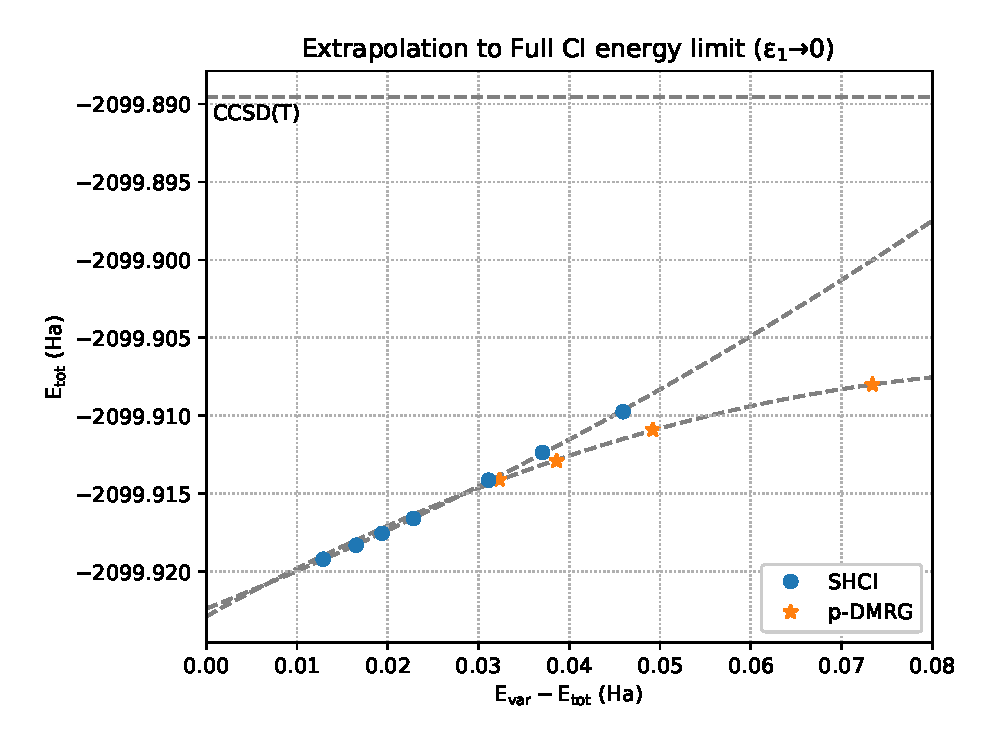
\includegraphics[width=\linewidth]{extrapolation/extrapolate.eps}
  \caption{Weighted quadratic extrapolation of the Cr$_2$ ground state energy.
  The weight of each point is $(E_{\rm var} - E_{\rm tot})^{-2}$.
  The extrapolated energy is $-2099.9224(6)$, where the uncertainty comes from the difference between linear extrapolation and quadratic extrapolation.
  The p-DMRG extrapolation and the CCSD(T) value are also shown.
}
  \label{fig:extrapolation}
\end{figure}

We extrapolate our results using a weighted quadratic fit~\cite{ChiHolOttUmrShaZim-JPCA-18}
and obtain for the ground state energy, $-2099.9224$~Ha as $\Delta E\to0$.
The weight of each point is $(E_{\rm var} - E_{\rm tot})^{-2}$.
Fig.~\ref{fig:extrapolation} shows the computed energies and the extrapolation.
We also perform a weighted linear fit and use the difference of the extrapolated values from the quadratic and the linear fits (0.6~mHa) as the uncertainty.
%If we look at the trends of the data points in Fig.~\ref{fig:extrapolation}, we can see that 0.55~mHa is a reasonable estimation of the uncertainty.
%In summary, the estimated full-CI energy of Cr$_2$ in the cc-pVDZ basis with active semi-core electrons is $-2099.9224(6)$~Ha.
In summary, the estimated full-CI energy of Cr$_2$ in the cc-pVDZ-DK basis with 28 correlated electrons and the relativistic X2C Hamiltonian
%(the rest of the electrons are frozen in
%Hartree-Fock orbitals)
is $-2099.9224(6)$~Ha.

\begin{figure}
  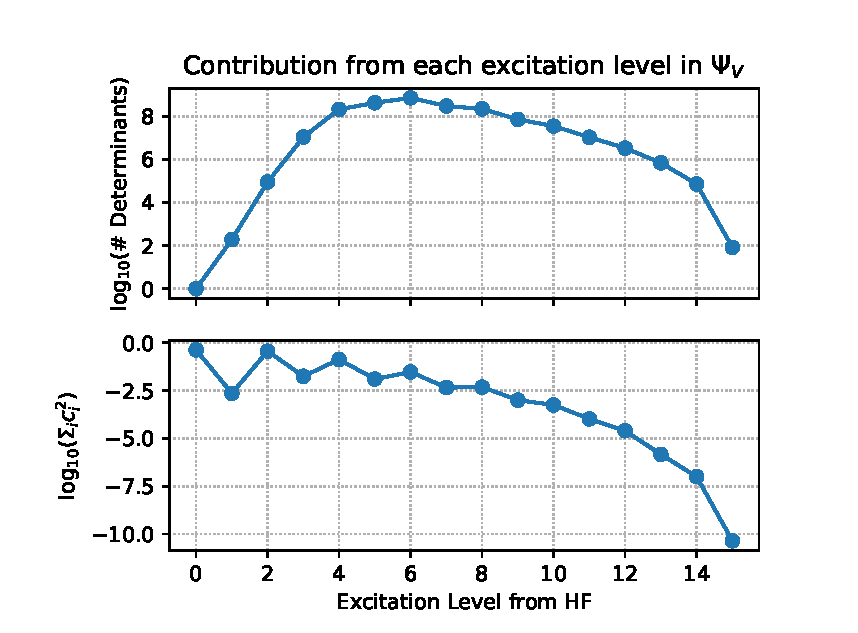
\includegraphics[width=\linewidth]{excitation/excitation.eps}
  \caption{Contribution from each excitation level to the variational wavefunction for Cr$_2$ with $2 \times 10^9$ determinants.
  Determinants with up to 15 excitations are present in the variational wavefunction.
%  {\color{red} Leave out the top plot, since sums of squared magnitudes is meaningful, but number of nonzero magnitudes is a meaningless quantity? Well, it does mean that there were several higher-order excitations that are more important than lower-order ones.}
}
  \label{fig:excit}
\end{figure}

We compare our result with DMRG and p-DMRG, which are the only essentially exact methods that have been applied to this large active space of the chromium dimer.
The DMRG calculations use up to bond dimension $M=16000$ and obtain an extrapolated energy of $-2099.9195(27)$~Ha (default schedule) and $-2099.9192(24)$ (reverse schedule)~\cite{GuoLiCha-JCTC-18}.
%These two values are similar to our most accurate data point but higher than our extrapolated result by 3~mH, which is about one standard error of the DMRG results.
These two values are similar to our most accurate data point but higher than our extrapolated result by 3~mH, which is about the estimated error of the DMRG results.
%The p-DMRG calculations use up to $M=4000$ and obtain an extrapolated energy of $-2099.9201$~Ha~\cite{GuoLiCha-JCTC-18}.
The p-DMRG calculations use up to $M=4000$ and extrapolated energy obtained from a linear fit is $-2099.9201$~Ha~\cite{GuoLiCha-JCTC-18}.
If instead, we perform a weighted quadratic fit (shown in Fig.~\ref{fig:extrapolation}), the extrapolated energy is $-2099.9225$~Ha,
in perhaps fortuitously good agreement with our result of $-2099.9224(6)$~Ha.  However, the extrapolation uncertainty is larger than the SHCI extrapolation uncertainty.
In contrast, the CCSD(T) energy is considerably higher.
%In summary, our extrapolated value agrees with DMRG's and p-DMRG's extrapolated results but we achieve a smaller uncertainty.

One of the merits of selected-CI is the ability to take higher-order excitations into account accurately.
To see the contribution from each excitation level we plot the number of selected determinants and the $\sum_i \left|c_i\right|^2$ versus excitation level in Fig.~\ref{fig:excit}.
Determinants with excitation levels up to 15 excitations are present in the variational wavefunction even though we are using optimized orbitals.
(Using Hartree-Fock orbitals, we expect that determinants with even higher excitation levels will be present.)
%This implies that truncating the CI or the CC at the double or the triple excitation level may not give reliable results for such strongly correlated systems.
This implies that truncating the CI expansion at the double, triple or quadruple excitation levels (which is the most that is usually done in systematic
CI expansions), will give poor energies for such strongly correlated systems.


% The smallest $\epsilon_2$ we use for the perturbative stage is $3\times10^{-9}$.
% Due to the stochastic nature of our algorithm, we do not know exactly how much perturbative determinants are in effect during our calculation.
% However, we can estimate the lower bound based on our largest pseudo stochastic run.
% In that run, we use an $\epsilon$ of $3\times10^{-8}$ and 457 batches, and we got about 39.3 billion determinants per batch.
% Hence, the total number of effective determinants for the pseudo-stochastic stage is 18 trillion, which is also the lower bound of the number of effective determinants for $\epsilon_2=3\times10^{-9}$.

% In this section, we use Fast SHCI to obtain the ground state energy of the Cr$_2$ dimer.
% Cr$_2$ is a well-known challenging system for electronic structure methods.
% We perform frozen core calculations with a bond-length of \SI{1.68}{\angstrom} in the cc-pVDZ-DK (28e, 76o), cc-pVTZ-DK (28e, 126o), and cc-pVQZ-DK (28e, 198o) basis.
% The largest Hilbert space contains more than $10^{42}$ determinants.
% We have studied Cr$_2$ before with SHCI but only with 12 active electrons~\cite{ShaHolJeaAlaUmr-JCTC-17}.
% With Fast SHCI, we can obtain much more accurate results on these bases by correlating 28 active electrons.

% \begin{table}[h]
%   \begin{tabular}{| c | c | c | c |}
%   \hline
%   Basis & $\epsilon_{\rm var}$ & $E_{\rm var}$ & $E_{\rm total}$ \\
%   \hline\hline
%   \multirow{8}{*}{cc-pVDZ-DK} & $2.00\times10^{-4}$ & -2099.799310 & -2099.887592(10) \\
%    \cline{2-4}
%    & $1.50\times10^{-4}$ & -2099.810487 & -2099.889577(09) \\
%    \cline{2-4}
%    & $1.00\times10^{-4}$ & -2099.824867 & -2099.889577(09) \\
%    \cline{2-4}
%    & $7.00\times10^{-5}$ & -2099.835878 & -2099.889577(09) \\
%    \cline{2-4}
%    & $5.00\times10^{-5}$ & -2099.845027 & -2099.889577(09) \\
%    \cline{2-4}
%    & $4.00\times10^{-5}$ & -2099.850520 & -2099.889577(09) \\
%    \cline{2-4}
%    & $3.00\times10^{-5}$ & -2099.857019 & -2099.889577(09) \\
%    \cline{2-4}
%    & Extrapolated & \multicolumn{2}{ c |}{-2099.889577(09)} \\
%    \hline
%   \multirow{8}{*}{cc-pVTZ-DK} & $2.00\times10^{-4}$ & -2100.037667 & -2099.887592(10) \\
%    \cline{2-4}
%    & $1.50\times10^{-4}$ & -2100.053072 & -2099.889577(09) \\
%    \cline{2-4}
%    & $1.00\times10^{-4}$ & -2100.073358 & -2099.889577(09) \\
%    \cline{2-4}
%    & $7.00\times10^{-5}$ & -2100.089210 & -2099.889577(09) \\
%    \cline{2-4}
%    & $5.00\times10^{-5}$ & -2100.102756 & -2099.889577(09) \\
%    \cline{2-4}
%    & $4.00\times10^{-5}$ & -2100.111002 & -2099.889577(09) \\
%    \cline{2-4}
%    & $3.00\times10^{-5}$ & - & -2099.889577(09) \\
%    \cline{2-4}
%    & Extrapolated & \multicolumn{2}{ c |}{-2099.889577(09)} \\
%    \hline
%   \multirow{8}{*}{cc-pVQZ-DK} & $2.00\times10^{-4}$ & -2100.142048 & -2099.887592(10) \\
%    \cline{2-4}
%    & $1.50\times10^{-4}$ & -2100.159753 & -2099.889577(09) \\
%    \cline{2-4}
%    & $1.00\times10^{-4}$ & -2100.182527 & -2099.889577(09) \\
%    \cline{2-4}
%    & $7.00\times10^{-5}$ & -2099.810487 & -2099.889577(09) \\
%    \cline{2-4}
%    & $5.00\times10^{-5}$ & -2099.810487 & -2099.889577(09) \\
%    \cline{2-4}
%    & $4.00\times10^{-5}$ & -2099.810487 & -2099.889577(09) \\
%    \cline{2-4}
%    & $3.00\times10^{-5}$ & -2099.810487 & -2099.889577(09) \\
%    \cline{2-4}
%    & Extrapolated & \multicolumn{2}{ c |}{-2099.889577(09)} \\
% %   HCI & 3TB & 145.0 & 0.000 \\
% %   \hline
% %   \multirow{2}{*}{SHCI} & 128GB & 14.5 & 0.010 \\
% %   \cline{2-4}
% %    & 32GB & 116.6 & 0.010 \\
% %   \hline
% %   \multirow{2}{*}{Fast SHCI} & 128GB & 3.7 & 0.009 \\
% %   \cline{2-4}
% %    & 32GB & 4.2 & 0.009 \\
%   \hline
  
%   \end{tabular}
%   \caption{Perturbation time for copper atom in cc-pVTZ basis with (19e, 88o) active space and 18.3 million variational determinants. HCI uses the usual deterministic perturbation. SHCI uses the semistochastic perturbation that solves the memory bottleneck. Fast SHCI uses the multistep batch perturbation that significantly improves the efficiency of SHCI, especially for memory constrained cases.}
%   \label{tab:Cr2}
% \end{table}

% Table~\ref{tab:Cr2} shows the variational and total energy for each $\epsilon_{\rm var}$ and each basis set.
% $\epsilon_{pt}$ in these calculations are all set to $0.001\epsilon_{\rm var}$.
% The extrapolated energy is obtained from quadratic extrapolation of $E_{\rm var}$ and $E_{\rm var}-E_{\rm total}$~\cite{HolUmrSha-JCP-17}.
% Fig~\ref{fig:ham} shows the extrapolation for each basis set.
% We can see from the figure that all the data points lie almost perfectly on the extrapolated curves, which proves the robustness of our extrapolation and the accuracy of the results.

% We also calculated the dissociation energy of Cr$_2$ in these bases at bond length \SI{1.68}{\angstrom} and compare it with other methods, including DMRG, AFQMC, MR-AQCC and DFT, and the most recent experimental values~\cite{vancoillie2016potential,purwanto2015auxiliary,simard1998photoionization}.
% Table~\ref{tab:Cr2} summarize the results.
% We can see that Fast SHCI results with 28 active electrons agree well with the experimental result from.
% DFT also gives good agreement to experiments with the appropriate choice of the functional.
% We can also see from the DMRG results that using 12 active electrons are not enough for getting the accurate energy of Cr$_2$.

\section{Conclusion}
\label{conclusion}
In this paper, we introduced our fast semistochastic heat-bath configuration interaction algorithm, an efficient and essentially exact algorithm for estimating the Full-CI energy.
We introduced a new Hamiltonian generation algorithm and a 3-step batch perturbation to overcome the bottlenecks in the original SHCI algorithm.
We also presented the key data structures and parallelization strategy, which are also crucial to the performance.
%The improved SHCI takes selected-CI to a whole new level and allows us to perform accurate quantum chemistry calculations on larger bases, with more electrons and achieve smaller errors than ever before.
These improvements allowed us to use $2 \times 10^9$ variational determinants, which is more than one order of magnitude larger than the $9\times 10^7$ determinants
used in our earlier SHCI calculation~\cite{ChiHolOttUmrShaZim-JPCA-18}, and two orders of magnitude larger than the largest variational space of $2\times 10^7$ determinants
employed to date in any other selected CI method~\cite{GarSceLooCaf-JCP-17}.

Future extensions of the method include going to yet larger variational spaces using a \emph{direct} method~\cite{Knowles1984,IvaRue-TCA-01}, wherein the Hamiltonian matrix is recalculated at each Davidson iteration and therefore need not be stored.
Although this increases the computational cost, the increase is not overwhelming because of the use of the auxiliary arrays introduced in this paper.
Other extensions include increasing the range of applicability of the method to larger systems by combining SHCI with range-separated density functional theory~\cite{Sav-INC-96},
and the use of SHCI as an impurity solver in embedding theories.
Applications include providing benchmark energies for a variety of organic molecules, as well as for transition metal atoms, dimers, and monoxides,
and providing calibration or training data for large scale methods,
%e.g., potential energy surfaces interatomic potentials for molecular dynamics, exchange-correlation energies for improving density functional approximations, and training data for machine learning.
e.g., to calibrate interatomic potentials for molecular dynamics and exchange-correlation functionals for density functional theory,
and to train machine learning based quantum chemistry solvers.
Calculations on the homogeneous electron gas are also underway.\\[1mm]
%Future works include applying SHCI to larger systems that have never been treated with essentially exact methods, making further improvements to the algorithm and extending its capability of calculating other quantities, such as the band structure.
%We are also looking into merging the merits of SHCI with other methods with good size-extensivity so that we can treat strongly correlated areas with SHCI accurately while avoiding the exponential scaling of CI between a large number of weakly correlated regions.

\begin{acknowledgements}
This work was supported by the AFOSR through grant FA9550-18-1-0095.
A.A.H was supported by the NSF under the grant ACI-1534965 and by the University of Colorado.
S.S. acknowledges the funding provided by the NSF through grant CHE-1800584.
%The computations were performed on the Bridges cluster at the Pittsburgh Supercomputing Center under NSF grant ACI-1445606,
%and on the Cooley and Theta clusters at Argonne National Laboratory.
%This work used the Extreme Science and Engineering Discovery Environment (XSEDE), which is supported by National Science Foundation grant number ACI-1548562. Specifically, it used the Bridges system, which is supported by NSF award number ACI-1445606, at the Pittsburgh Supercomputing Center (PSC).
The computations were performed on the Bridges computer at the Pittsburgh Supercomputing Center supported by NSF grant ACI-1445606, as part of the XSEDE program supported by NSF grant ACI-1548562,
and the Argonne Leadership Computing Facility (ALCF) at the Argonne National Laboratory.
\end{acknowledgements}

% \appendix
% \section{Implementation Details}
% % the \\ insures the section title is centered below the phrase: AppendixA

% Text of Appendix A is Here

% \section{\\Title of Appendix B}
% % the \\ insures the section title is centered below the phrase: Appendix B

% Text of Appendix B is Here

%\bibliographystyle{apsrev}
\bibliographystyle{apsrev4-1}
%\bibliographystyle{jchemphys}

\bibliography{main,hci,umrigar,toulouse,chan,needs}
%\bibliography{hci}

\end{document}
%
% ****** End of file apssamp.tex ******
